\documentclass{hasel_thesis}

\thesisType{Bachelor}
\date{\today}
\title{Motivating effective breaks for knowledge workers with Break  Scheduler }
\subtitle{Bachelor Thesis}
\author{Marinja Principe}
\home{Niederhasli} % Geburtsort
\country{Switzerland}
\legi{18-740-910}
\prof{Prof. Dr. Thomas Fritz}
\assistent{Dr. André N. Meyer}
\email{marinja.principe@uzh.ch}
\url{<url if available>}
\begindate{19.09.2022}
\enddate{19.03.2023}
\graphicspath{{images/}}

\begin{document}

\maketitle

\frontmatter

\begin{acknowledgements}
\end{acknowledgements}

\begin{abstract}
This is an abstract.
\end{abstract}

\begin{Summary}
This is the Summary.
\end{Summary}
    

\tableofcontents
\listoffigures
\listoftables
\lstlistoflistings

\mainmatter
\chapter{Introduction}
%Introduction: genau, hier kommt die Motivation und Zusammenfassung vergleichbarer Forschung, um den Gap zu zeigen, anschliessend eine Zusammenfassung deiner Arbeit, Evaluation und Erkenntnisse, sowie Zusammenfassung der Contributions 

%- Importance of breaks
% %- why do we need breaks
% - How does it influence knowledge workers
% - Examples of papers which have shown breaks are important
%Why do we need breaks?
%What is a break? (vacatation, ..
\textcolor{red}{Motivation and description of work}

\section{Motivation}

\textcolor{red}{Motivation}
 \begin{comment} 
- Background and context of the research problem
- Research problem and object description ives
- Research Methodology

\end{comment}






Most knowledge workers face a highly fragmented workload and many commitments, which can cause stress and dissatisfaction. This can lead to burnout or problems for the organization \cite{Elkin.1990}. Therefore, it is important to learn more about the recovery process of employees. Various studies \cite{Largo-Wight.2017},\cite{KimS.ParkY.&Niu.2017} have shown that regular breaks can significantly reduce work-related stress.  In addition, regular breaks can reduce physical discomfort \cite{Waongenngarm.2018}, but also help people stay focused \cite{Ariga.2011} \cite{Bloom.2014} and thus keep productivity high throughout the workday. Trougakos et al. ~\cite{Trougakos.2009} propose to differentiate breaks in a systematic manner into vacation breaks, breaks between work days (such as weekends), and breaks within work days. While the effects of vacation breaks are usually short-lived, short, regular breaks within the workday have greater value for recovering a worker's personal and physiological resources.
Some studies investigated how to find the right time for a break to increase productivity and well-being. Kaur et al. \cite{Kaur.2020} explored the finding of opportune moments for knowledge workers to take a break, using affect, workstation activity and task data. Their study demonstrated an accuracy of 86\% using their approach for predicting opportune moments. In addition, several commercial approaches and tools that support reminders for taking breaks exist and are already widely used \cite{Alghamdi.2020}, for example, the Pomodoro technique \cite{Cirillo.2006} or the 20-20-20 rule \cite{Min.2019}. Packer et al. \cite{Packer.2021} showed that micro-breaks have a restorative effect on well-being and focus.  However, finding the timing of the micro-break is essential as shown by Kaur et al. \cite{Kaur.2020}. Nevertheless, different studies \cite{KimS.ParkY.&Niu.2017} \cite{Berman.2007} have demonstrated that there is no one "perfect" break schedule that suits everyone. While some people prefer and benefit more from having regular short breaks at the coffee machine, others prefer to go for a walk during their lunch break. Therefore, finding opportune moments for a good break and knowing how best to spend them remains a challenge. 

Since each person has only a limited amount of personal resources, it is necessary to understand how to spend them and, more importantly, how to recover them. The theory of resource depletion \cite{BaumeisterR.F.BratslavskyE.MuravenM.&TiceD.M..1998} states that each person has only a limited amount of "personal resources" that can be consumed, but also recovered, depending on the activity. Activities that consume resources are so-called chores. On the other hand, activities that restore resources are called respite breaks \cite{Trougakos.2009}. Whether an activity restores or consumes resources varies from person to person. This indicates that break activities are key to a good break. But when, how long, and with what activities should a good and effective break be spent? 


%One of the most effective ways to promote physical and mental health is to incorporate small positive habits  into everyday life \cite{Taylor.2005}. Since many adults spend a large portion of their day at work, it can be valuable to consider the time they spend at work for incorporating small positive habits. Most knowledge workers face a highly fragmented workload and many commitments, which can lead to stress and dissatisfaction. Different studies \cite{Largo-Wight.2017},\cite{KimS.ParkY.&Niu.2017} have shown that regular breaks can significantly reduce work-related stress.  In addition, regular breaks may reduce physical discomfort \cite{Waongenngarm.2018} but also help to stay concentrated \cite{Ariga.2011} \cite{Bloom.2014} and, thus, keep productivity high throughout the workday. 
%But when, how long and with which activities should a good and effective break be spent? 




%- Good / Effective breaks
 % - Definition of a break
 % - what is a good break what is a bad break?
 % - How can we influence breaks (timing, duration and activities)
 %    - show paper with different activities and show that it is important how to spend break time

 % - what is already done in relation to breaks?
 %    - speak about google tool, activity study etc.

 % - show there is not tool incorporating all 3 aspects
 % - Explain the goal and approach of this thesis

Before we look into the definition of a \textbf{good break} it is important to define the term break. \cite{Trougakos.2009} defines a break as a time in which work-related tasks are not expected nor required to be done. In other words, a break is a time when the owner can decide how to spend it, in order to achieve a good break. In this work, we are using the definition of a good break by \cite{Trougakos.2009}. A "good break" is a break that recovers the personal resources of an person. On the other hand a "bad break" will drain the anyway limited resources. If an activity recovers or drains resources is depending on two main aspects: The amount of effort, which is used to fulfill this activity and whether it is enjoyable for the person. Good ways of spending breaks are to spend time in nature, relax or perform physical activity \cite{Bloom.2014} \cite{Largo-Wight.2017}.  As shown by Kim et al \cite{KimS.ParkY.&Niu.2017}, there are different types of breaks. They are divided into relaxation, nutritional, social, and cognitive micro-breaks. Each of these groups has a different goal and therefore a different use. For example, stretching exercises and naps can contribute to relaxation, while short conversations with work colleagues about non-work related topics improve social support. These activities also affect the duration of a break. But it's not just the activity that affects the duration of a break. Different techniques, such as the Pomodoro technique or the 20-20-20 technique, recommend different break duration.

Overall, existing approaches considered static break schedules and did not let users personalize the break timing to individual preferences and needs (e.g. \cite{Henning.1997} \cite{Cooley.2013}), or did not  support users in identifying how to best spend their breaks, to facilitate recharging and recovering (e.g. \cite{Kaur.2020}). 
The goal of this work is to develop a personalized break planner that supports users in finding the opportune time for an activity and deciding on an activity in order to develop good/effective break habits. 


The following questions will be explored and answered through a user study:

-	[Awareness] RQ1: How can self-reflection and nudging increase knowledge workers' awareness about their existing break habits and their personal resources, such as energy, attention levels or physical well-being?

Awareness is an important aspect of change. First, e person needs to be aware of their action before they can evaluate whether their actions need change or not. Therefore the Break Scheduler wants to be able to raise awareness of its user's personal resources, such as energy, attention and physical well-being. Input data for raising awareness of personal resources are limited to self-reports. The rule-based system and nudging should help the user to evaluate their behaviour and suggest better alternatives. The goal is also to find specific features of the solution which can increase knowledge workers' awareness of break habits.


-	[Impact] RQ2: Can a personalizable break scheduler support knowledge workers' identification of good break activities and what is the impact on their break habits and ability to recharge personal resources during breaks?

When awareness is raised the user can act on it and generate an impact. For each break, the Break scheduler suggests a timing, duration and activity which was evaluated by the rule-based system. The impact of the rule-based system and the different analysis features in to be evaluated in the user study. To evaluate the impact, a pre-questionnaire will be compared with the user data of the tool, as well as the post-questionnaire. As the Break Scheduler should enable users to find good breaks, how it can enable the user to find good breaks and if there exist activities beneficial for different people.


-	[Tool] RQ3: Which aspects of the personalizable break scheduler prototype are most helpful, and are there design improvement opportunities?
In the end, the implementation of the Break Scheduler will be discussed. Potential advantages and disadvantages will be discussed, in order to create a personalizable tool which helps the user to identify good break habits and raise the awareness of their resources. The fisability of it incorporation into the daily life and andling will also be discussed.


\section{Description of Work}
\textcolor{red}{description of work}
- Structure of the thesis


%
 %Factore for a "good break" \cite{Bloom.2014}
 %- Recovery process
 %- health (physical and mental)
 %- well-being
 %- job performance
 %- creativity

 \chapter{Background} \label{background}
 \begin{comment} 
 - Definition of a Break
 - Personal Resources and Physiological Capacities
 - Self-Reporting /self-Experimenting

 
\end{comment}

This section will establish a common understanding of the theory used for the presented solution. First, the background of personal resources and physiological capacities will be examined, followed by an introduction to work recovery. Finally, the definition of a break used for this thesis and an overview of different break types are shown.

\section{Personal Resources and Physiological Capacities}

\begin{comment} 
 - what are personal resources, what are physiological capacities (done)
 - why is it important (done)

 
\end{comment}
Personal and physiological resources are a key concept of the presented application, which is why they will be discussed in detail in this section. The counterpart of resources is job demand which is also influenced by job control. Both of these values go hand in hand, therefore both are important concepts to look into in more detail. Why resources and the balance of resources are essential will be shown in the last section of this chapter.

\subsection{Definition of Personal Resources and Physiological Capacities}
In the study by Baumeister et al. \cite{BaumeisterR.F.BratslavskyE.MuravenM.&TiceD.M..1998}, they define \textbf{personal resources} as a limited set of resources that enable a person to complete various activities during the day. The amount of resources varies from person to person. This concept has been applied in multiple areas of psychology and organizational behaviour. While some studies focus on specific factors such as energy or stress, personal resources encompass various aspects. These include (but are not limited to) factors such as attention, energy, well-being, creativity, decision-making, and social contacts. Each person has a limited amount of personal resources available daily, so it is essential to know how to recharge them. 

\textbf{Physiological Capacity}, on the other hand, is a limited resource beyond which a person is physically unable to continue without rest. An example would be sleep or food. Each person has a limit to how long they can physically go without sleep or food. To restore physiological capacity, each person must sleep, eat, or drink. Exhaustion of physiological resources usually leads to serious health consequences \cite{Trougakos.2009}. At this point, it is essential to mention that the two resources (personal and physiological) are not entirely independent.
Some studies \cite{Meijman.1998,Hobfoll.1989, Hobfoll.1998} do not separate personal resources from physiological capacity. These theories use the definition of limited resources, which is crucial for the next chapter on recovery.

Meijman and Mulder's \cite{Meijman.1998} focus on the effort-recovery model, which deals with workers' efforts and their work management. The central concept is that a worker's work effort leads to work overload and decreased personal resources. According to them, recovery can only begin by taking time away from the overall work demand. This shows the importance of the recovery process and awareness of personal resources.

Hobfoll's \cite{Hobfoll.1989, Hobfoll.1998} conservation of resource theory compares stress and well-being and investigates the relationship between them. They were able to show that the loss of resources is more noticeable than the recovery / the gain of resources. This enhances the point that it is suggested to prevent a resource deficit proactively.

Both studies include the concept of work demands that require effort or resources to be completed. The following section discusses the concepts of job demand and job control.



\subsection{Job demand and Job Control} \label{job_control}
The term \textbf{Job demand} refers to the features (physical, psychological, social etc.) of a job that require effort and, therefore, have a specific resource cost to complete them \cite{Trougakos.2009}. Examples of job demands are a heavy workload or time pressure. Previous studies can show that a high work demand affects the well-being \cite{Sonnentag.2003} of the person as well as their needed recovery time \cite{Sonnentag.2006}. A high job demand often leads to the feeling of time pressure. On the other hand, this leads to a depletion of resources as the increased demand requires more effort to complete all the tasks. As the time pressure is already high, the time for breaks and recovery will be relatively short or cut altogether, leading to less or no time for recovery while using more resources than available. This is also why many people with a high job demand engage in more chore activities such as work or running errands.
Compared with people with low job demands, short breaks for people with high demand may not be sufficient to recover from the resource deficit created over time. In such cases, only a more significant period, for example, some days off, can restore their resources effectively. However, when the resources are refilled, it is essential to pro-actively and continually engage in activities which restore the personal resources to avoid a deficit again.

The job demands-resources model \cite{BakkerA.B.DemeroutiE.DeBoerE.andSchaufeliW.B..2003b, DemeroutiE.BakkerA.B.NachreinerF.andSchaufeliW.B..2001a} also includes a similar notion of demand. According to their definition, job demands refer to aspects of work concerning physical, psychological, social or organizational factors. Each task uses a particular effort and skills, which leads to a sum of demand costs, e.g. physical or psychological costs. When the employee can not recover from this job demand, the demand can turn into job stressors \cite{Hobfoll.1998}. Such stressors can lead to physiological (e.g. cortisol level increase) or/and psychological symptoms (e.g. fatigue)\cite{Sonnentag.2022}. Resources are essential to balance each person's needs and work demands. As defined in the job demands-resources model, Job resources refer to physical and psychological aspects required to finish tasks, reduce job demand and achieve personal growth. Hence, not only are resources necessary as a balance for job demand but also for the development of each person. Job resources have the potential for motivation, leading to high engagement and performance. Therefore, job resources also have an intrinsic, motivational role \cite{Bakker.2007}.

If this balance between demand and resources is off, the work demand can become a stressor. In addition, people with fewer job or personal resources are more prone to resource depletion because abundance also consumes resources \cite{Trougakos.2009}. 

\textbf{Job control}, on the other hand, refers to the ability of each employee to influence their job activities \cite{Trougakos.2009} and enable them to take decisions. Many studies were already able to show that high job control benefits the employee's well-being \cite{Daniels.1994, Jackson.1983}. High job control has an advantage in two ways. First, employees with high job control are flexible to take breaks or switch activities when tired, which helps them recharge their resources flexibly to their needs. Secondly, each employee can structure their day to fit their needs, for example, by joining a yoga course during the lunch break. To summarize, employees with high job control are 
a) more likely to take a break when it is needed and 
b) more flexible in the selection of the activity, as they can vary their break durations.
On the other hand, studies have shown that employees with high job control and no formally scheduled breaks often do not take any breaks and overwork themselves \cite{McLean.2001}. They fail to take a break when needed, so they only take breaks when their resources are already meagre. If they then engage in breaks activities, it is not enough anymore for them to take short breaks but they need an extended break. Especially employees with less repetitive work (e.g. knowledge workers) can benefit from high job control \cite{Trougakos.2009}. Job control also affects the perception of certain activities. Let us consider the example of working during lunchtime. A person with a high job control decides to work during lunchtime, knowing that they have the control to stop whenever needed. Compared to a person with low job control, whose employer asks to finish a task before leaving, the perception of the person with high job control will likely not be as draining as the other.

But what happens when the equilibrium between an individual's personal resources and the demands and control within their job becomes imbalanced?

\subsection{Consequences of Personal Resource Levels}
The consequences of different levels of personal resources will be discussed in more detail to underline the importance of the proactive management of personal resources. 
Other research has found a relationship between stress and depletion of resources \cite{Sonnentag.2001}. Additionally, Trougakos and Hideg \cite{Trougakos.2009} suspect that low resources lead to high emotional exhaustion. They propose the following explanation. When personal resources are low, people are more prone to stress and less able to deal with it. This theory will also be covered by one of the most influential stress theories by Lazarus and Folkman \cite{Lazarus.1984}, which state that personal and social resources play an important role when dealing with stress. According to Lazarus and Folkman, specific tasks will be perceived as a stressor when already coping with stress, whereas when resources are high, they will be more likely to be perceived as a challenge.
Furthermore, Lazarus and Folkman \cite{Lazarus.1984} distinguish two types of coping mechanisms: Problem- or emotion-focused strategies. People with low resources prefer to distance themselves from a problem as they can not deal with it now. On the other hand, people with high resources are more likely to tackle the issues and try to solve them, which will change the current situation, leading to a likely better position.
Last but not least, one \cite{Trougakos.2009} argues that the performance during the day depends on the assigned focus, which depletes the resources during the day. It is necessary to restore personal resources to keep the performance during the day high. When this is not done, the performance can degrade\cite{Trougakos.2009}, as these resources are limited.

As stated above, the consequences of personal resources are significant for different reasons, including the employee's well-being and job performance. Therefore it is crucial to understand how to recover personal resources despite the daily work demand.
 

 \section{Work Recovery Research}
  \begin{comment} 
 - why are we looking at recovery for work --> many knowledge workers are stressed and recovery is key
  - How can we recharge this resources
 - Different ways of recovery: 
    - organisational
    individual -->breaks
\end{comment}
As seen in the last section, personal and physiological resources are limited and differ from person to person. A deficit of these resources can lead to depletion of work or/and decrease the mental or/and physical well-being. The recovery of these resources is, therefore, a fundamental concept for mental and physical well-being. Sonntag et al. define recovery as an “unwinding and restoration process during which a person’s strain level has increased as a reaction to a stressor, or any other demand returns to its prestressor level” \cite[p.366]{Sonnentag.2017}. Usually, such stressors are generated by work demands, including negative state characteristics. This negative state can be characterized by high arousal as anger or anxiety, but it can also be characterized by low arousal as exhaustion, depression or fatigue \cite{Sonnentag.2022}. As restoration is done by eliminating the demand for a certain period of time \cite{Trougakos.2009}, the recovery can only start when the job demand has ended, including the psychological detachment from work. 
However, if this demand can not be decreased, as the person is mentally still present, or demand remains due to other stressors; no recovery can take place, and the load reactions accumulate over time. This leads to a higher work demand and a high resource depletion since an abundance of resources also consumes resources \cite{Trougakos.2009}.


One potential counteract for depleted resources is \textbf{motivation} \cite{Bandura.1986}. Work motivation is defined as the will to achieve a certain goal \cite{Locke.2004}. Locke \cite{Locke2000} has shown that job performance depends not only on one's skills or abilities but also on motivation. As every job task leads to a certain goal, the perception of the goal is crucial. The Goal-Setting Theory by Latham and Locke \cite{Latham.1991} states that when a goal is challenging and more advanced, it will lead to a greater outcome. More challenging goals often lead to bigger rewards, such as pay or a higher reputation. Therefore, employees often feel that even if their resources are low, it will be beneficial for them to continue and achieve the goal, increasing their focus and effort. The motivation helps them strive towards their goal and temporarily compensate for low resources. On the other hand, if a goal is not be perceived as "worthy" more energy is needed to complete the task or it will not even be completed at all \cite{Trougakos.2009}. Muraven and Slessareva \cite{Muraven.2003} conducted a study which can show that a depleted person can continue working on tasks which are perceived as essential or beneficial for them or others. They can show that depleted people continue working on self-control tasks which they believe are helpful to others, whereas people who do not believe the tasks will help others do not continue. Additionally, people who thought they could personally benefit from the task performed better than people who did not. In summary, Muraven and Slessareva \cite{Muraven.2003} state that depleted people are motivated for a task when the benefits of the outcome are higher than the associated cost of their resource depletion. On the other hand, a clear direction and goals can have an impact on well-being and stress levels when resources are low. Previous research can show that role ambiguity is positively related which stress and even emotional burnout \cite{Posig.2003}. Role ambiguity will be defined as the lack of clear goals and/or directions. A depleted person needs clear goals and direction to know where to invest their remaining energy to achieve the goal. Additionally, when resources are already low, formulating and defining new clear goals might be challenging. When speaking about motivation, it is essential to differentiate between intrinsic and extrinsic motivation. Intrinsic motivation refers to having a choice, for example, when a person autonomously and out of their own volition defines a goal. This motivation inherits interest and is enjoyable. On the other hand, extrinsic motivation is forced and controlled. They lead to external validation as rewards or avoiding punishments \cite{Ryan.2000}. Intrinsic motivation employees will perform better as the tasks are more enjoyable and, therefore, easier to complete.

Another important definition when looking into work recovery is the definition of \textbf{chore and respite activities} \cite{Trougakos.2009}. According to their definition of resource depletion \cite{BaumeisterR.F.BratslavskyE.MuravenM.&TiceD.M..1998}, each activity can consume or restore personal resources, depending on different factors and preferences. 

Activities that consume more resources than they can recover are called \textbf{chores}. They continue draining resources and fail to restore personal resources. Such activities can negatively affect work performance or well-being. Sonntag \cite{Sonnentag.2001} was able to show that such activities primarily represent continuing with work in different ways, for example, switching tasks, domestic tasks or running errands and generally require an increased regulation of behaviour. These activities are mostly not enjoyed by the person, resulting in resource depletion. It is essential to state that the perception if an activity is a chore is highly dependent on the subject's perception. An example would be cooking, which some people enjoy leading to the recovery of personal resources, while others do not, leading to a depletion of their resources.


On the other hand, activities that restore these sources are called \textbf{respites}. To recover, activities need to be low effort, preferred choice, or enjoyable \cite{Trougakos.2009}. As shown in the sections above, high resources positively affect job performance and well-being. Therefore respite activities are essential for job performance and well-being too. Trougakos and Hidge \cite{Trougakos.2009} specify two characteristics for a respite activity: the amount of effort and the degree on how much it was their preferred choice. A low effort helps the person to reduce the demand and uses fewer resources to do the activity, resulting in a higher resource outcome. High-effort activities mostly increase demand, which is disadvantageous for the demand reduction necessary for recovery. A high effort can be balanced by the degree of preferred choice. These activities can aid in the recovery of depleted resources as they are enjoyable or energize the user. They generate a positive feeling and well-being. Exercise is an example of a high-effort but preferred choice activity, as the activity uses a lot of energy but leaves the person with a positive feeling and a higher mental and physical well-being. These two factors define if an activity is perceived as a respite or chore activity. However, as seen in the given an example, the balance between them is crucial and differs from person to person. However, it is suggested that respites are selected for break activities, as they restore personal resources, whereas chores are advised to be avoided. This shows that break activities are essential factors for a beneficial break.

As a common understanding of personal resources and how to recover resources is established, the definition of a break can be looked at in more detail.


\section{Definition of a Break}

A work break is defined by \cite{Trougakos.2009} as a period of time when no work-related tasks are expected or need to be completed. It is suggested that breaks should be spent doing activities with low demand on resources, enabling the user to recover them. Moreover, the recovery ability of the break depends on how the break time is spent. The activity of a break is therefore key. This includes various types of breaks such as vacations, weekends, breaks at the end of the day, and breaks during work, including micro-breaks. In order to understand the advantage and disadvantages of these types of breaks, it will be further elaborated.


Lounsbury and Hoopes \cite{Lounsbury.1986} define vacation as a period of time "when a person is not actively engaged in his or her work. It is a time when a person is free to pursue other interests, and therefore a time when the work situation may become less important compared to other areas of experience such as family and personal leisure" \cite[p. 393]{Lounsbury.1986}. The goal is to regain energy to be more productive during work time. It has been shown by \cite{Westman.1997, Westman.2001} that vacations reduce stress and lower burnout levels. Additionally, employees are more likely to engage in respite activities, which are relaxing and enjoyable, leading to positive emotions and recharging of personal resources \cite{Fritz.2006}. Unfortunately, these effects wear off within days or weeks after returning to work again. This means that vacations have only a short-term positive impact on stress levels \cite{Fritz.2006}.


Weekends and end-of-day are mini-vacations between work days that allow workers to relax and engage in other non-work related activities. Unfortunately, there are not yet as many studies that specifically look at weekends and their benefits to workers, but the studies that do exist show that the lack of time off can lead to lower well-being or burnout \cite{Fritz.2005}. Weekends promote rest and well-being through restorative and stimulating activities, preferrable with low demand. Additionally, engaging in favourable and low-demand activities at the end of the day leads to greater recovery. Weekends and end-of-day can be used to recharge personal resources, but only when invested in respite activities. Resources are depleted if they are used for chore activities such as longer working hours or running errands.


The first study of breaks during the working day goes back to Mayo in 1933 \cite{Mayo.1933}, in which a very general form was studied. The best-known types of breaks during the day are coffee or lunch breaks. A particular type of with-in-day breaks are microbreaks, defined as really short breaks, e.g., less than 10 minutes \cite{BennettAndrewA.GabrielAllisonS.CalderwoodCharles.2020}. Several studies have already examined the benefits of such breaks and how they can contribute to the recovery of personal resources. For example, just 5 minutes of stretching can help combat muscle fatigue that typically occurs after 40 minutes. Such research mainly focuses on the interval of the breaks, their timing, and their duration. Only a few studies specifically focus on the activity during those breaks. However, it was found that break activities during the workday affect emotions and their recovery process, showing that enjoyable and restful activities provide greater recovery \cite{Trougakos2008}. 

When considering further research, one can find a relatively clear common message: To understand the recovery process, one needs to consider the activity conducted during a break, not depending on the break type. Generally, as already shown in the recovery research, activities with low demand tend to have greater recovery and activities which fail to reduce the demand tend to have negative consequences. Especially for with-in-day breaks, it is often the case that employees can not emotionally detach themselves from work and therefore struggle to recover during breaks. In the case of vacations or weekends, it is often easier for employees.



\chapter{Related Work} \label{related_work}
%-	Das «theoretical background» chapter nennen wir meist “Related Work”, aber solche Details können wir dann später anschauen, wenn auch klarer ist, ob es noch einen theoretischen Hintergrund braucht. Hier wird dann sicher auch ein Kapitel wichtig sein zum Thema wie Wissensarbeiter:innen arbeiten, und weshalb Pausen wichtig/gut sind, und weshalb es schwierig ist, diese zu Timen, Managen, und geeignete Aktivitäten zu finden. Dh. Du kannst dann in den Subkapiteln (detaillierter als in der Intro) aufzeigen, was es schon gibt, und wo dein Ansatz anknüpft bzw. was neu ist
\begin{comment} 
- Overview of previous research on knowledge worker motivation and breaks
- Relevant theories and concepts related to knowledge worker motivation and breaks
- Previous studies and research works on the impact of breaks on productivity and well-being
\end{comment}

To understand existing work in the area of this thesis, the next chapter will examine the importance of breaks for knowledge workers and the promotion of breaks in their work environment. Additionally, already existing studies on the characteristics of effective breaks will be discussed.

\section{The Importance of Breaks for Knowledge Workers}
\begin{comment} 
Preventive breaks can help to reduce phisical disconfort, but most of the time knowledge worker only take breaks when it is alreaddy to late. cite Frequent short breaks...

Also add something to work cultur
\end{comment}

Knowledge work has become increasingly important in today's world. As automated machines take over routine and manual labour, the work of knowledge workers has become a critical factor in the economy \cite{Oskarsdottir.2022}. As noted by Oskarsdottir et al. \cite{Oskarsdottir.2022}, knowledge workers' well-being and personal resources are critical factors in their productivity. They divide the related factors into two groups: Internal factors, which include well-being and personal resources, and external factors, such as salary, job design, organization and culture.
In this thesis, we are only concerned with internal factors, specifically knowledge workers' well-being and personal resources.

One of the most effective ways to promote physical and mental health is to incorporate small positive habits into daily life \cite{Taylor.2005}. Since many knowledge workers spend a large portion of their day at work, it can be helpful to use the time they spend at work to establish small positive habits. Most knowledge workers face a highly fragmented workload and many commitments, which can lead to stress and dissatisfaction. Several studies \cite{Largo-Wight.2017, KimS.ParkY.&Niu.2017} have shown that regular breaks can significantly reduce work-related stress. In addition, frequent breaks can reduce physical discomfort \cite{Waongenngarm.2018} and help stay focused \cite{Packer.2021}, thus keeping productivity high throughout the workday.
As work requires energy and effort, it drains the energy level of knowledge workers and can influence their physical and mental well-being. After a certain period, it is necessary to recharge the resources used for accomplishing the work tasks \cite{Sonnentag.2006}. For most knowledge workers, this recovery process only starts each day after working hours. As shown in the background section \ref{background}, weekends and end-day recovery are essential for the well-being of each person. Still, with-in-work breaks can help knowledge workers proactively keep their resources high and prevent the depletion state, which needs even longer breaks to recharge. They are also beneficial for job performance as they can increase the assigned focus to each task \cite{Trougakos.2009}. 


\subsection{Promoting breaks in workspaces}
To incorporate with-in-day breaks, knowledge workers need to have a workspace which enables their employees to take breaks. One key factor for a beneficial break environment in the workspace is high job control. Especially in the area of knowledge workers, which are involved in several projects with different agendas and deadlines, it is essential to have flexible schedule breaks, and restorative phases \cite{Trougakos.2009}. As discussed in the background section \ref{background}, knowledge workers mostly have high job control, leading to the flexibility to take breaks and the risk of overworking. Having a tool supporting knowledge workers in maintaining their flexibility while engaging in healthy break routines is essential. Some studies, such as that of Kaur et al. \cite{Kaur.2020}, use effect, job activity, and task data to examine which moments are opportune for knowledge workers to take a break. They can predict the right time with 86\% accuracy. However, other, more commercial tools support break reminders and are already widely used \cite{Alghamdi.2020}, for example, the Pomodoro technique \cite{Cirillo.2006} or the 20-20-20 rule \cite{Min.2019}. Some of the already existing solutions and studies will be discussed in more detail in the next section.
 


\begin{comment} 
Desired benefits were shared, but subjective
When asked to explain what makes a break good and/or
successful, 112 respondents (76%) referred to a desired mental
state upon returning to work. Examples include breaks that
“cleared my mind”, where they returned “refreshed”,
“refocused”, “relaxed”, or “recharged”, or that the break
“lowered my stress.” An overall theme was that workers return
from a successful break feeling ready to work. 

Kaur et al. \cite{Kaur.2020} explored the finding of opportune moments for knowledge workers to take a break, using affect, workstation activity and task data. Their study demonstrated a 86\% accuracy of the approach for predicting opportune moments. In addition, several commercial approaches and tools that support reminders for taking breaks exist and are already widely used \cite{Alghamdi.2020}, for example the Pomodoro technique \cite{Cirillo.2006} or the 20-20-20 rule \cite{Min.2019}. Packer et al. \cite{Packer.2021} showed that micro-breaks have a restorative effect on well-being and focus.  However, finding the timing of the micro-break is essential as shown by Kaur et al. \cite{Kaur.2020}. Nevertheless, different studies \cite{KimS.ParkY.&Niu.2017} \cite{Berman.2007} have demonstrated that there is no one "perfect" break schedule that suits everyone. While some people prefer and benefit more from having regular short breaks to the coffee machine, others prefer to go for a walk during their lunch break. Therefore, finding opportune moments for a good break and knowing how best to spend them remains a challenge. 
\end{comment}




\section{Existing Studies on the Characteristics of Effective Breaks}
Important research was already done by many studies in the area of breaks. The most relevant for this thesis will be discussed to get a common understanding of different approaches.


\subsection{Timing of breaks}
% - what have other studies already shown
% - what is their approach
% - what can I learn in finding good time slots for breaks
% - Are there different types of people with different timing breaks
% - What are the factors influencing the timing? (input variables?)
Most of the studies done are looking into the break timing and duration of a break. A solution to find opportune moments for breaks at work was done by Kaur et al. \cite{Kaur.2020}. Using effect, workstation data and task information to conduct whether it is an opportune moment for a break or a task switch. Their accuracy timing is up to 86\%. However, this study only looks at the time when a break should be started but not the duration nor the activity even though many studies have shown that the activities are key for an effective break. They also differ between taking a break and switching tasks. When a person is stuck on a problem but the attention level is still high enough, they propose a task switch instead of a break.

Another approach is a tool called BreakSense \cite{Cambo.2017}. BreakSense is a mobile application which detects through Bluetooth if a person left his workplace. When it was sensed the person got up, small activities will be suggested which can be done in the office place. The goal is to incorporate small breaks to increase physical movement during work. Instead of suggesting timing, BreakSense detects when the knowledge worker is anyway not working and adds some small physical activities to it.

There are different tools like Flow (cite website) or TimeForBreak \cite{luo.2018}, which provide simple timers, for focus durations or break durations to follow the Pomodoro technic \cite{Cirillo.2006}. The user can define the duration for which he wants to focus on work or take a break and when the time is finished the user will be reminded. Such a simple timer can have a positive effect on the user as the user does not need to remind taking breaks or need to check the time spend on a task. However, these tools only incorporate the timing of a break and the duration, but not the activity.


\subsection{Duration of the break}
\begin{comment} 
- what have other studies already shown
- what is their approach
- what can I learn in finding good time slots for breaks
- Are there different types of people with different timing breaks
- What are the factors influencing the duration? (input variables?)
- Is it correlated with the timing?
\end{comment}

Most of the already existing work does focus on the timing, however, as part of their study, important information on the break duration was found. The study of Epstein et al. \cite{epstein.2016t} conducted that the average break duration was 22.9 minutes. They also state the relation between activity and the duration of a break. While breaks outside prolonged a break, necessary breaks (as going to the toilette), mostly shortens the break duration. Additionally, digital breaks most of the time took longer than intended, whereas breaks outside or necessary mostly took less than anticipated.

\subsection{Activity during the break}
\begin{comment} 
- what have other studies already shown
- what is their approach
- Are there overall good activities? or is it personal
- Are there different types of people with different needs for activities?
- What are the factors influencing the activities? (input variables?
\end{comment}

Although there are already some studies on the timing and duration of a break, there is surprisingly less work on activities and the recovery process during a break. The study of Sonntag et al. \cite{Sonnentag.2022} looks at two approaches to studying the recovery process.

One approach focuses on the \textbf{activity during a break}. As defined by Trougakos and Hideg \cite{Trougakos.2009}, activities that consume personal sources are called chores, leaving the person with fewer personal resources than before the activity was practised. On the other hand, activities that restore these sources are called respite breaks \cite{Trougakos.2009}. Whether an activity restores or consumes resources depends on the person.
As discussed in the background section \ref{background}, two main factors influence a respite break: effort and enjoyablity\cite{Trougakos.2009}. Engaging in activities that the person does enjoy could lead to a positive experience. On the other hand, needing a lot of motivation to engage in an activity which is not so enjoyable causes a decrease in resources. Therefore finding enjoyable activities has a high value, as there are barely any resources needed to do them, but they recharge a lot of resources. Which activities are considered enjoyable and which aren't is very personal.
\textbf{Individual differences} influence the experience and appraisal of the activities. One individual factor is the extraversion of a person. The definition of extraversion by McCrae and John \cite{McCrae.1992} states that it is the degree to which a person is talkative, assertive and energetic. Highly extroverted individuals may recharge their personal resources while engaging in social activities, such as eating lunch with other people. At the same time, introverted individuals label such an activity as a chore. These activities drain more energy from them than they can recharge. Introverted people may benefit more from having lunch alone, enabling them to recharge their social energy and restore their personal resources. Another interesting point is that previous research could find that people with a higher extraversion compared to people with a lower extraversion have a more positive appraisal tendency \cite{Gallagher.1990, Hemenover.1996}, leading to a higher coping ability \cite{Penley.2002}. Additionally, they experience more happy emotions, which helps them to deal better with daily stressors \cite{Gallagher.1990}. Although it is eventually more difficult for introverted people to regain their personal resources, past research can show that individuals mostly stay in occupations and organisations which fit their personalities and therefore enable introverted people to recharge their personal resources \cite{Johansson.1970, Schaubroeck.1998}. Thus, individual differences play a significant role when looking into the activities.


The other approach focuses on \textbf{psychological experiences}. Psychological experiences refer to a person's mental state when being on a break and how they experience the break. Sonntag and Fritz \cite{Sonnentag.2017} use the following terms to determine the recovery experience: psychological detachment from work, relaxation, mastery, and control. Most research attention goes into the psychological detachment from work, which focuses on freeing the mind from work thoughts and gaining distance to the work during free time. Relaxation focuses on activities that calm a person's body and mind. On the other hand, mastery refers to overcoming challenges and learning, wheras, control refers to self-agency to decide what to do in non-work times. These four recovery experiences can be shown empirically, and conceptional \cite{sonnentag.2007}. Therefore, they must be considered when achieving a good and beneficial break.


When looking at break activities, self-reporting has been proven effective in different studies \cite{Bloom.2014, epstein.2016t}. Epstein et al. \cite{epstein.2016t} conducted a study by building a desktop application which gives insights into the break habits of the user in relation to their productivity using self-reports. They can show that the pre-break productivity significantly influenced the selected activity. When productivity was rated low, participants tended to take digital breaks such as checking emails, whereas when productivity was high, they tended to take necessary breaks such as going to the bathroom. Their data shows that the required break length is around 5min, whereas the break duration for going outside is around 10min. Therefore, the duration is dependent on the activity.



\chapter{Personalized Break Scheduler Design Approach} \label{design_approach}
%Anschliessend ist es wichtig, nicht gleich mit dem Tool/Implementierung zu beginnen, sondern deinen Approach zu bzw. die Grundkonzepte erklären. D.h. 3.1 und 3.2 könnten wahrscheinlich hier reinpassen; die genauen Konzepte können wir dann aber auch noch besprechen.


\begin{comment} 
Contrary, studies have shown that employees which have a high job control and no formally scheduled breaks, often do not take any breaks and overwork themselves \cite{McLean.2001}. They fail to take a break when needed, so they only take breaks when their resources are already really low. If they then engage in breaks activities, mostly it is not enough anymore to take short breaks but need an extended break.
- notification is good so that people do not forget to take breaks (take positiv of high job demand but elimit the bad of not having scheduled breaks)

II. Design Overview

Explanation of the design process and methods used
Presentation of the user interface and functionality of the Personalized Break Scheduler
Discussion of the design goals and requirements

\end{comment}

As seen in the chapters \ref{background}, the limitation of personal resources determines different factors of knowledge workers' mental and physical well-being \cite{Trougakos.2009}. However, many studies only consider the timing or the duration when looking at breaks and do not consider the activities during these breaks, as shown in section \ref{related_work}. Some studies focus on the activities but only on dictating specific activities to compare their effectiveness. The approach of this thesis is a software focusing on helping its user to find beneficial break activities and helping to raise awareness of personal resources and their usage. Supporting this goal, the following three key objectives were defined:

\begin{tcolorbox}[colback=white!5!white,colframe=black!75!black]
 •	Improve awareness of users on their existing break habits and their effectiveness

•	Enable users to self-reflect on their personal resources, such as attention, energy and physical well-being.

•	Empower users to identify good break activities that restore their personal resources
\end{tcolorbox}



From now on, this software will be referred to as the Break Scheduler. The Break Scheduler is developed to enable users to reflect on their personal resources and break habits to find beneficial breaks during work hours. It is essential to state that the main concept is not about dictating the perfect break schedule for the user but rather enabling the user to analyse his break habits and personal resources.

\section{Awareness of Personal Resources and Break Habits}
Improving awareness and enabling the user to self-reflect on their personal resources are two of the main objectives of the Break Scheduler. As shown in different studies \cite{GRANT20083}, self-reflection is a commonly used strategy to enable the user to raise awareness and take proactive actions. Therefore, different self-reporting measurements are used in the Break Scheduler to improve awareness. First, users will be asked to rate their personal resources each morning and evening. In the morning, they will be asked how many personal resources they have currently measured in percentage. Rating personal resources present itself as a challenge. Therefore, a percentage rating should help the user to define his own measurement scale. In the evening, each user rates their used personal resources, including the daily job demand in percentage. The primary value of this self-reflection is to see the relationship between personal resources over the day and how they change over the week. The reported morning and evening values need to be visualised for the user to reflect on their value over the week.

Not only is the awareness of personal resources essential, but also the awareness about break-taking habits. Therefore the second measurement is to ask the user about their existing break habit knowledge. In order to force the participant to reflect on their break habits and state that taking regular breaks is not a luxury, but a necessity, each user will be asked to state their preferred break interval, which is the time between breaks when a user is focused and working, and also their break duration. The existence of breaks is a given but still enables users to define their preferred interval and duration. This personalisation of the interval and duration allows the Break Scheduler to adapt to its user's specific needs. Another measurement in raising the awareness of breaks will be done by scheduling them into the user's primary calendar so they and others can plan the daily schedule with the breaks in it. Again, the breaks are not scheduled during free time but, in advance, incorporated into the user's schedule. Scheduling breaks have only a limited advantage, as breaks are often forgotten, as discussed by \cite{McLean.2001}. A reminder prevents the user from forgetting about breaks, a problem that knowledge workers with high job control face, as discussed in the job control section \ref{job_control}.

\section{Definition of the 3 Key Aspects of a Break }
 In order to empower the user to define good break habits and find beneficial break activities, the Break Scheduler will proactively suggest breaks, which are planned in advance into the user's calendar. When scheduling a break, the Break Scheduler focuses on three main aspects: Timing of a break, duration of a break and break activities. The following subsections will consider and discuss these three values in more detail.

\subsection{Timing of breaks}
As shown through several studies \cite{Largo-Wight.2017} \cite{KimS.ParkY.&Niu.2017}, it is important to schedule regular breaks, but the preferred break interval can vary from user to user. Thus, the proposed approach will start with a fixed break interval, which the user can define and adjust. This interval will be corrected and personalised based on user preferences over time. In order to enable the user to find a fitting break interval, a simple rule-based calculation was defined, which will be explained in the implementation chapter \ref{rule-based-method-implementation}.

It is essential that breaks are not scheduled during meetings, thus interfering with a user's work schedule. Therefore the time of breaks must be adjusted to the user's personal calendar. Otherwise, they can not participate in any breaks. This feature will be achieved by synchronising the personal calendar and the Break Scheduler. Additionally, all planned breaks will be saved in the personal calendar, which helps a user to remember his planned breaks when planning the rest of his work. A positive side effect is that other company members may have access to the user's calendar and could try not to schedule short-notice meetings into your planned breaks or motivate them to join some of the breaks.

\subsection{Duration of the Break}
Different techniques, such as the Pomodoro and 20-20-20 approaches, suggest different break duration. However, depending on the time of day and activity, the break duration may differ, e.g., a lunch break compared to a coffee break at 9 am. Based on users' self-reports, the approach aims at finding a more optimal duration for each user. Each evening the user will reflect on the break duration and state if it was good, too long or too short. The rule-based system will adjust the duration according to the user's input. As the lunch duration can differ from day to day, the user will also need to enter their preferred lunch duration for the next day. The lunch break can differ from day to day, as people can have lunch meetings, a high work demand leading to a shorter lunch break, or have already made plans for lunch. The Break Scheduler considers the input of the evening report when scheduling breaks for the next day. On the other hand, the duration also depends on the activity. Depending on the duration, the group of possible activities should be adjusted.

\subsection{Activity during the Break}
As discussed in the background section \ref{background}, the activities pursued during a break significantly impact the benefit of the break. The term beneficial or "good" must be defined to find beneficial breaks. In this thesis, a "good" or "beneficial break" is referred to as a break which leads to more personal resources than the user had before participating in the activity. As long as the net value is positive, it will be a good break. However, if the break has a net negative value as the activity uses more personal resources than it can regain, it will be defined as a "bad break". Such breaks should be avoided as they do not help recharge personal resources. 
The more scientific word for "good" and "bad" activities are respite and chore activities, as stated in the background section \ref{background} \cite{Trougakos.2009}. The following section will define how the Break Scheduler evaluates if a break activity is a respite or a chore. Users' preferences and self-reports on their experience with the activity should be incorporated to personalise the suggestions for break activity. 

\section{Evaluation of the Break} \label{evaluation_break}
As discussed in the background section \ref{background}, whether a break is a chore or respite depends on the net value of personal resources before and after the break. The Break Scheduler will therefore evaluate whether a break is beneficial or not from the user's input before and after the break. The user reflects on the state before the break has started and does reflect again on his resources directly after the break. To enforce the evaluation, each participant will receive a reminder when a break should start. Additionally, the report can only be done during the break; afterwards, it is not possible anymore. This design choice prevents the "I can also do it afterwards"-syndrome, which could falsify the input. As it is hard to state the current personal resources, it is even harder to quantify them after some time has passed. Therefore this report can only be done at the time of the break. As the concept of personal resources is hard to quantify, the Break Scheduler uses three central values to state the user's personal resources: Energy, attention and physical well-being. As these quantifiers need to be stated before and after each break activity, the number of asked values must be as small as possible, giving a brought insight into the personal resources. 

\textbf{Energy}: energy resources are also defined as personal resources at work by Klijn et al. \cite{klijn.2021}. They define energy as a multidimensional construct encompassing physical, emotional, cognitive, and psychological factors. According to Klijn et al., energy is considered a personal resource enabling its holder to deal with the work demand. Additionally, they also found that energy is positively related to well-being and job satisfaction and negatively related to burnout and stressors. Considering these factors, energy is one of the quantifiers for the Break Scheduler.

\textbf{Attention capacity}: attention capacity is defined by Fried and Aricak \cite{Fried2014} as the ability to assign attention resources to complete tasks. They consider attention a personal resource as its owner can use them to cope with work demands. On the other hand, the authors can show that attention capacity can play an essential role in the user's well-being and how to deal with stressors.


\textbf{Physical well-being}: As discussed in the background section \ref{background}. The physiological capacity of each person is limited, and after a certain level, the person is forced to recharge (as the example of eating or sleeping). A deficit in these values mostly leads to serious health issues \cite{Trougakos.2009}. In some definitions, physical capacity will also be added to the personal resources and is therefore important for Mental well-being. Different studies show that sleep significantly influences a person's performance and stress level \cite{Rosekind.2010, Choi.2018}, proving that physiological resources are important factors to consider. Previous studies can show that physical and mental health are interlinked \cite{Doan.2022}, proving the importance of incorporating physical well-being as a crucial factor when determining whether a break is beneficial. 

These three quantifiers do not claim to complete the whole range of personal and physiological resources. These values are needed to cope with work demands and are part of personal resources. Even though they do not cover the whole range of personal resources, they are practical values in giving insights into the user's current state. Since each person has an individual and subjective perception and evaluation of these three values, the rule-based system does not look at the values per se but at the difference between the values before and after the break. This removes the individual definition of the scale and focuses only on the change before and after the break. 

\textbf{Enjoyability}: Another essential factor when looking at how beneficial a break is, is the \textbf{preferred choice}. As discussed in the background section \ref{background}, the benefit of a break can be measured by two factors: effort and preferred choice. If an activity is enjoyable, it will generate more personal resources and can also balance out the fact that it is high effort, as the example of working out shows. The fourth value counting into the break evaluation is, therefore: "How enjoyable was the activity?" which will be asked after each break.

\textbf{Experience value:} all these four values will be included in the experience value of the break activity. The experience value state how beneficial the activity was for the user in the past. The higher the value, the better. If the value is positive, it is stated as a respite activity; if it is negative, it is a chore activity. How to calculate the experience value will be shown in the implementation of the rule-based method in section \ref{rule-based-method-implementation}.

\section{Rule-based Method}
The rule-based method is the central heart of the Break Scheduler. This part suggests to the user the three main factors of a break: timing, duration and, most important, the activity. It is important to mention again that the rule-based method will generate a suggestion and does not claim to dictate the break timing, duration or activity. It should support the user in finding good break habits while adjusting to their needs.


\subsection{Timing and Duration of Breaks}
The rule-based system starts with a static rule, such as the 50-10 rule, which a user will define before starting the first Break Schedule. The user can define his preferred break interval and duration, which will be used for the timing and duration of the schedule and will be adjusted over the next few days. Additionally, they are adjusted depending on the time of day. For example, there should be no breaks at the end of the day to ensure the finishing of tasks, or when it is lunchtime, the break duration should be extended. For the timing and duration calculation, the Break Scheduler has two types of data: static and non-static values. 

Static data are the defined break interval as well as the break duration. They will be defined at the beginning when the break scheduler starts for the first time and can 1) be manually adjusted when needed or 2) adjusted over the week as part of the personalisation. Static values do not drastically change daily and are less influenced by daily circumstances but rather stay the same. These values are fixed when the system starts scheduling breaks for the day. 

Non-static data will be defined every evening before the schedule is generated. They include the start of the day, end of the day, lunch break duration and, of course, the calendar events for the next day. These data is day specific as they can change frequently. Before creating the Break Schedule, a user must confirm or adjust the start and end of the next day and their lunch duration. As the Break Scheduler is synchronised with the personal calendar, a user does not have to enter the calendar data.


\subsection{Activity during the Break}
In order to detect "good" break activities, each activity has an experience value. This value should sum up how the activity was rated in the past. Activities with a higher experience value should be chosen for future breaks. How the experience value is defined is shown in the implementation of the rule-based method in section \ref{fig:rule-based_method}. 

In order to enable the personalisation of the user, each user will be asked to select activities they want to experiment with.
Certain activities can be grouped as they have similar characteristics. The Break Scheduler should also consider such a signed in beneficial categories of groups. Not only the category but also the daytime can influence whether a break activity is considered beneficial or not. That is why each of the activities has assigned categories. All defined categories are shown in figure \ref{fig:categories}, according to Kim et al. \cite{KimS.ParkY.&Niu.2017}.

\begin{figure}[htp]
    \centering
    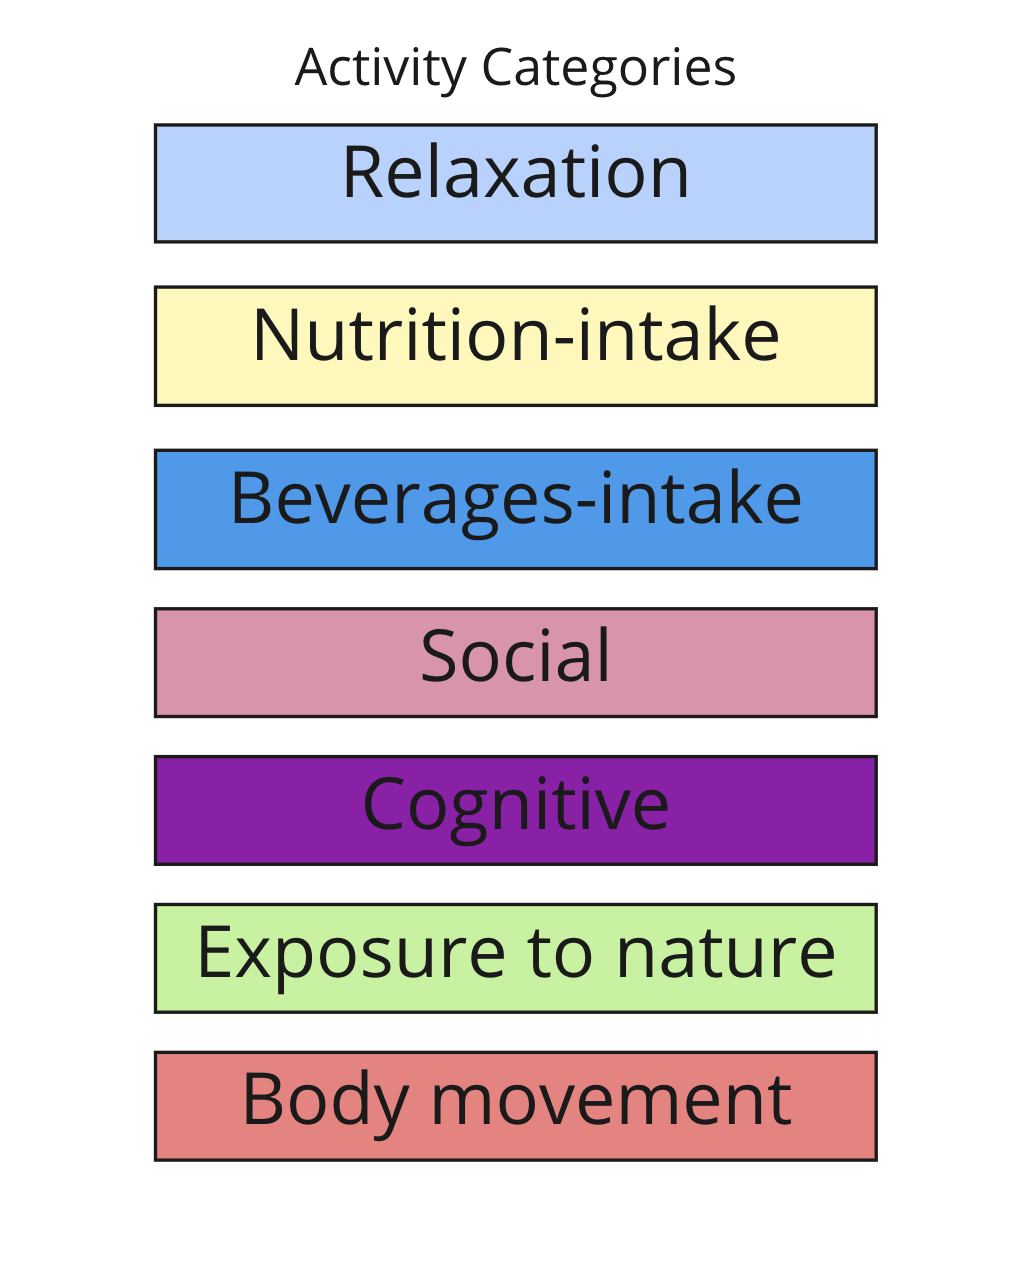
\includegraphics[width=4cm]{hasel_thesis/images/categories.png}
    \caption{Break Scheduler Categories according to Kim et al. \cite{KimS.ParkY.&Niu.2017} }
    \label{fig:categories}
\end{figure}

These categories will be used to analyse the different aspects of activities, such as body movement or nutrition intake, and also include the daytime for suggesting beneficial activities. Each of these categories, therefore four assigned values: an overall sum of experience value, a morning sum of experience value, a lunch sum of experience value and an afternoon of experience value. When selecting an activity, it is essential to ensure 1) the selection of the past beneficial breaks and 2) the incorporation of the daytime into specific groups of activities. This will be done by combining the categories with the daytime experience values and the activity experience values. At the start of using the Break Schedule, it is also essential to suggest activities that have not yet been tried to ensure each activity was tested before suggesting the most beneficial one. More details about the detailed implementation will be discussed in the implementation of the rule-based method in section \ref{fig:rule-based_method}.

When selecting an activity, the experience value and duration are vital, as not each activity can be completed in different break durations. Therefore, the rule-based method should also consider the duration when selecting an activity. The choice of activity also depends on the daytime. At lunch, an activity from the "Nutrition intake" category must be selected, whereas morning or afternoon activities from the highest-ranked category will be selected. 

Suggesting only one activity can feel restrictive, which could decrease the user's motivation to take breaks. Therefore, a random activity will be chosen from the whole activity list in addition to the suggested activity. This mechanism adds some randomness to the activity selection process and helps to reduce bias which can appear when only the activity with the highest experience value is suggested. Each user will have a suggestion and a random activity to choose from before starting their break. 




\chapter{Implementation}
\begin{comment}
4.2, 4.3 und 4.4. gehören in 5 – hier geht es ganz konkret darum, wie du die Key-Features/Themes aus dem Approach programmiet/umgesetzt hat. Hier stellst du deinen Break Scheduler vor
\end{comment}

In this chapter, the implementation of the key features which were defined in the Design Approach section \ref{design_approach} will be looked at. The first section will discuss the system architecture to provide the reader with a comprehensive system overview before diving into the specifics. After that, the main focus is placed on the user interface implementation and the functionalities of the Break Scheduler.

\section{System Architecture}
\begin{comment} 
Describe the overall system architecture, including the components, modules and the relationships between them
Components: User interface, Rule-based system, Google API, Microsoft API and SQLITE DB
\end{comment}
The Break Scheduler desktop application is a standalone electron application mainly written in Typescript. It is built with Electron \cite{electron}, a popular framework for cross-platform desktop applications, to ensure the publication of the desktop app on the three main operating systems: macOS, Windows and Linux. The application has four main components: user interface, rule-based system, calendar integration, and database. In figure \ref{fig:architectur} connection of these four components is visualized.


\begin{figure}[htp]
    \centering
    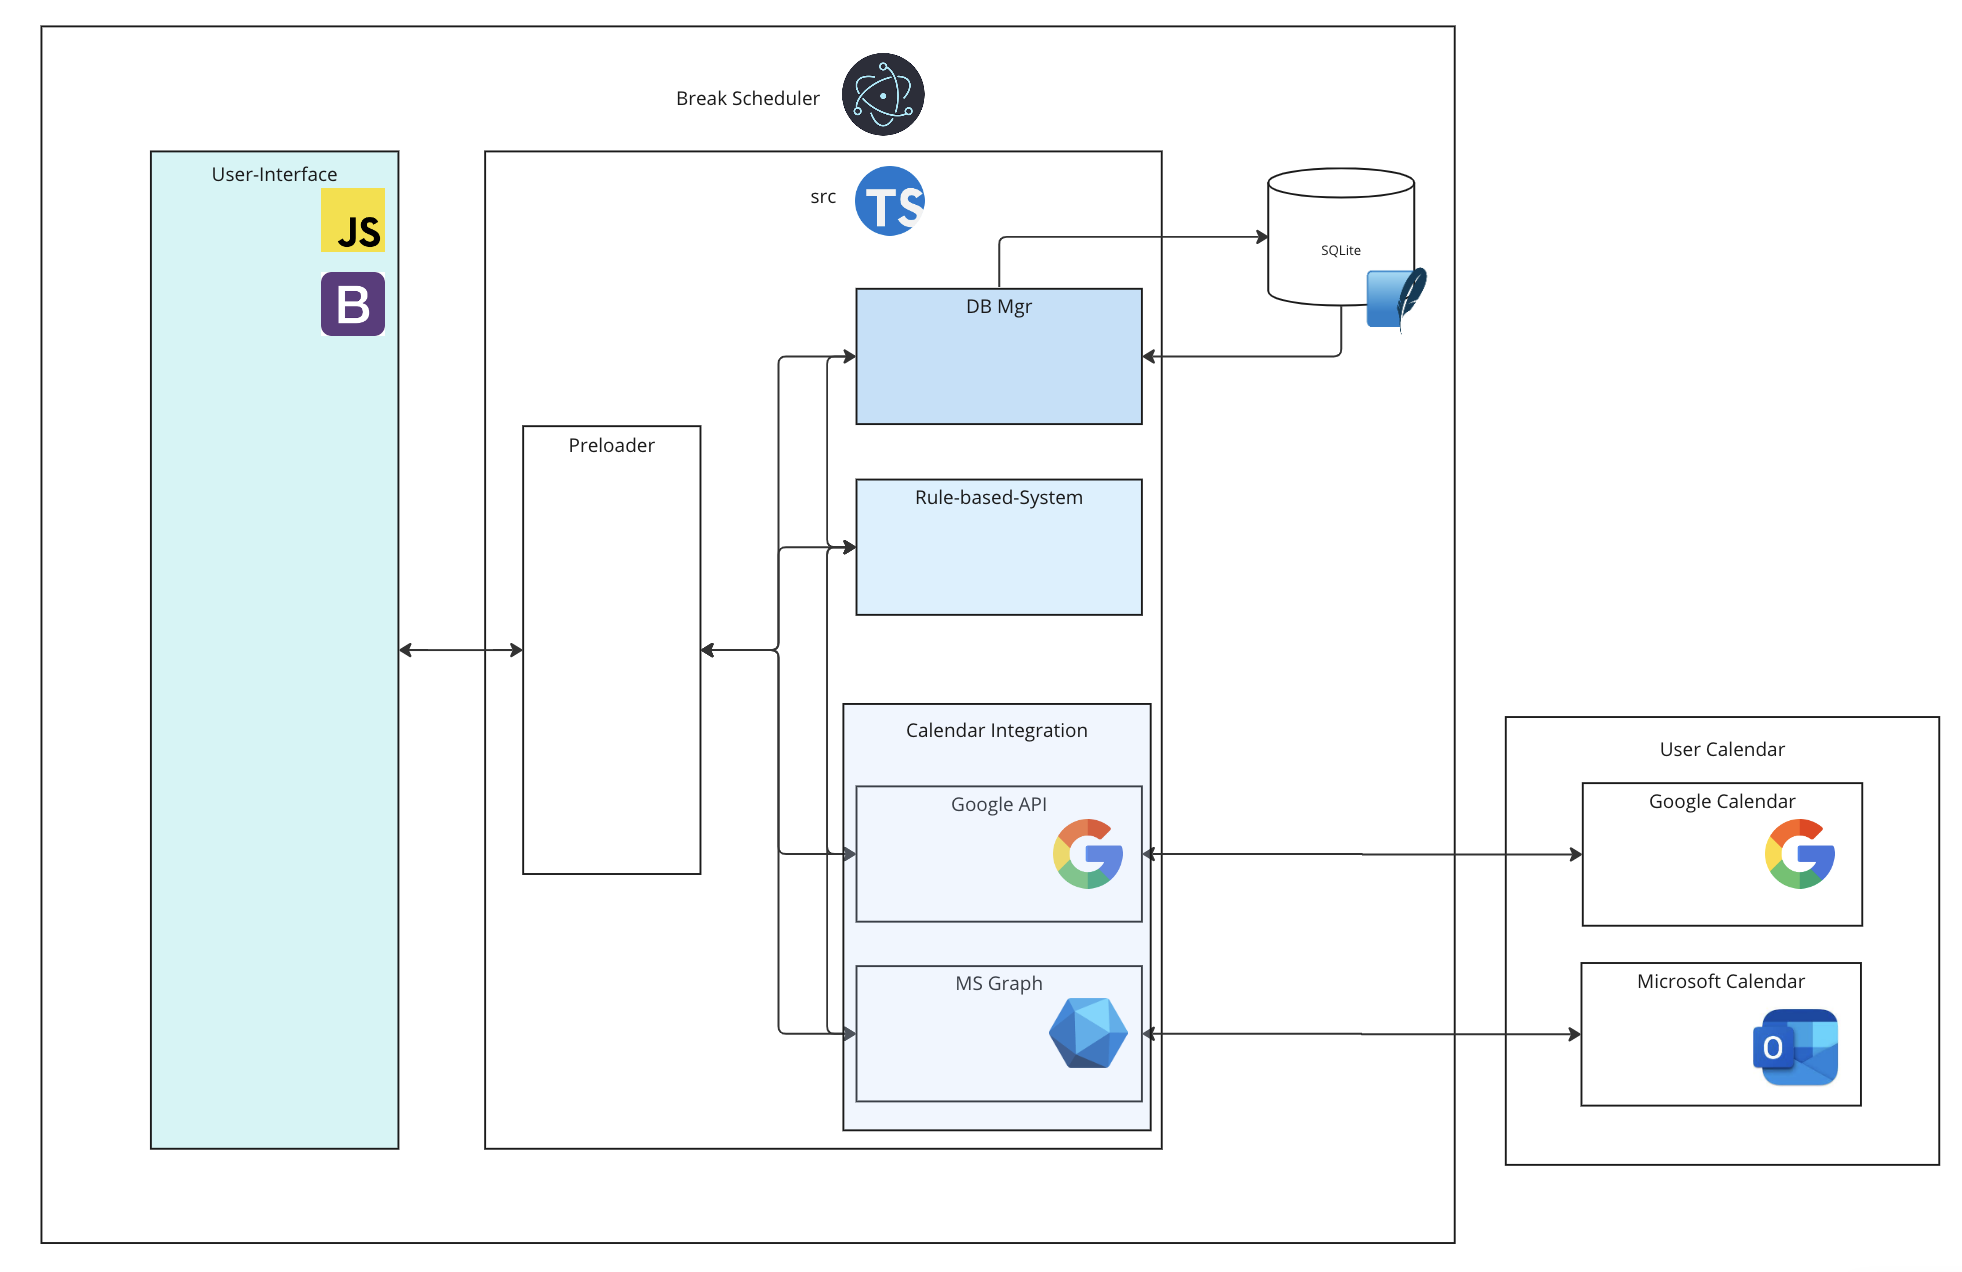
\includegraphics[width=14cm]{hasel_thesis/images/architectur.png}
    \caption{Break Scheduler architecture}
    \label{fig:architectur}
\end{figure}


\textbf{User Interface:} A key aspect of every application is the user interface and a self-explanatory design. The user interface's primary goal is visualising the generated data and enabling users to adjust and reflect on them. Different predefined dashboard templates were used when designing the interface to ensure the user experience and human-centred interaction (HCI). The User Interface section \ref{interface} will show details of the user interface and its specification. All data from and to the user interface will be transferred through the preload file, as suggested by the electron's inter-process communication (IPC).


\textbf{Rules-Based System:} The rule-based system is the heart of the Break Scheduler. It generates the Break Schedule and performs the calculation for the experience values. Its implementation will be discussed in section \ref{rule-based-method-implementation}.


\textbf{Calendar Integration:} To support the user to plan breaks around their work schedule, calendar integration is crucial. Users have two possibilities, they can either connect the Break Scheduler with their Google calendar or their Microsoft calendar. For this, the Break Scheduler is connected to the Google API and the Microsoft Graph API. Each minute the Break Scheduler synchronises the calendar with the user calendar and checks for changes. Additionally, when the application generates the schedule, the application will post all suggested breaks into the personal account, enabling proactive planning of the breaks. More implementation details are discussed in section \ref{calendar_integration}.


\textbf{Database:} The database used for the Break Scheduler is a simple SQLite database, which is well-suited for storing small amounts of data within a desktop application. This file is stored locally on the user's machine. The advantage here is that the user owns all of his stored data, and no one else can access it without their consent. Within this database, the initial settings, the activity and category values, as well as all self-reports are saved. This information is needed for the rule-based method to work. For this study, additional information is stored in the database, such as logs and scheduled breaks.

In the next section, the user interface design and the key functionalities, including the rule-based system, the calendar integration, and the database, will be discussed.

\section{User Interface Design} \label{interface}
\begin{comment} 
Description of the layout, navigation, and overall look and feel of the application
Explanation of how the design meets the user needs and requirements
Discussion of the user testing and feedback received during the design process

Description of the visual design elements, such as color scheme, typography, and layout
Explanation of the navigation structure and how the different pages and features of the application are organized and accessible to the user
Overview of the design of specific components, such as buttons, forms, and icons, and how they contribute to the overall user experience
Discussion of how the design supports the user's goals and meets their needs, such as ease of use, accessibility, and overall aesthetic appeal
Discussion of how the design has been tested and validated with users, including any user research or testing methods used


\subsection{Initial Break Plan}

- How do i generate the initial break plan
- What different people do we have
- How can the user adjust this plan
- What is the theory behind it


 
The Break Scheduler starts with an initial break plan. To achieve this plan, the user will be asked to define their key values, such as the preferred break interval and break duration. They can also decide to go with the default, 50-10, as various papers recommend. (add paper here!). Additionally, they will be asked to fill out specific settings questions as if they would like to include a lunch break and state the lunch break duration. A list of predefined break activities will be shown, from which the user can choose what to incorporate and what not. This will help to cancel already break activities which are not feasible or preferred. After this initial questionnaire, the break schedule will be defined for the first time. All activities in every category are same likely to be chosen for the breaks as there is no data yet. 

\subsection{Adapting to User's Needs}

- How is the system working?
- what are trigger values?
- what is the weight of the trigger values?
- Why did i choose this concept? (Show theory)

The generated break schedule is synchronized with your chosen calendar interface (Outlook or Google Calendar). This synchronization allows the Break Scheduler to ensure no breaks are scheduled during meetings. Additionally, all generated breaks will be added to your calendar, and a reminder will be displayed for morning and evening reports. A crucial point for the Break Scheduler is the integration of the tool into the user's work environment and the integration with tools already in use, so it does not require much maintenance in the tool itself. For this reason, all break adjustments are made in the personal Outlook or Google calendar, synchronized with the Break Scheduler. The user can adjust the start time and duration or delete the break if new appointments come up during the day.
The goal is to help the user find their best fit and allow manual adjustments to stay flexible throughout the day by working with a single tool, their personal calendar. 

At the end of each day, the user will be asked to rate the break interval and duration. If the timing was rated as good, the interval and duration will stay the same for the next day. However, when the duration or timing is too short or too long, it will be adjusted relative to the current value and will be extended or respectively reduced. This enables the user to learn more about their fitting break duration and interval and enforces the user to reflect on the break habit in the evening. This easy yet effective mechanism enables Break Schedule to adjust the user's needs and raise awareness.

Before and after each break, there is a brief self-reflection in which the user assesses their energy and attention levels and physical well-being. These insights and an assessment of the activity yield the experience value of that break. This value is added to the activity as well as the overall and daily category value. The experience value will help the scheduler find good and effective breaks in the next iterations. However, The suggested breaks are only suggestions. The user does not need to perform this activity. The rule-based system suggests one activity and one randomized activity from the whole list. The user can select one of the two. If both do not fit his needs, he can always choose an activity from the entire list, enabling the user to adjust to his current needs. The selected activity is the one which will be rated and will get the assigned experience value.

The setup described above has two personalizing factors. First, the rule-based system adjusts all three key values of a break, timing, duration and activity, over time. The timing and duration will be adjusted each evening when rating the interval and duration of the break. Additionally, depending on the user's calendar, the break timing and duration will be adjusted to fit the day. The selection of the activities will be adjusted through the experience values accumulated during the work day. Secondly, all three key values of a break can be adjusted by the user, enabling them to adjust the scheduled breaks to the current needs and changes during the day.

\end{comment}

The user interface is an essential factor of the Break Scheduler, as the application should enable users to reflect on their data with the help of different visualisations. When designing the interface, different predefined dashboard templates \cite{startAdmin}, \cite{codyhouse}, \cite{radiance}, and \cite{nicepage} for the generation of the self-reports 
were used to ensure the user experience and human-centred interaction (HCI). However, adjustments and the definition of the user flow needed to be made to fit the user's needs.

\begin{figure}[htp]
    \centering
    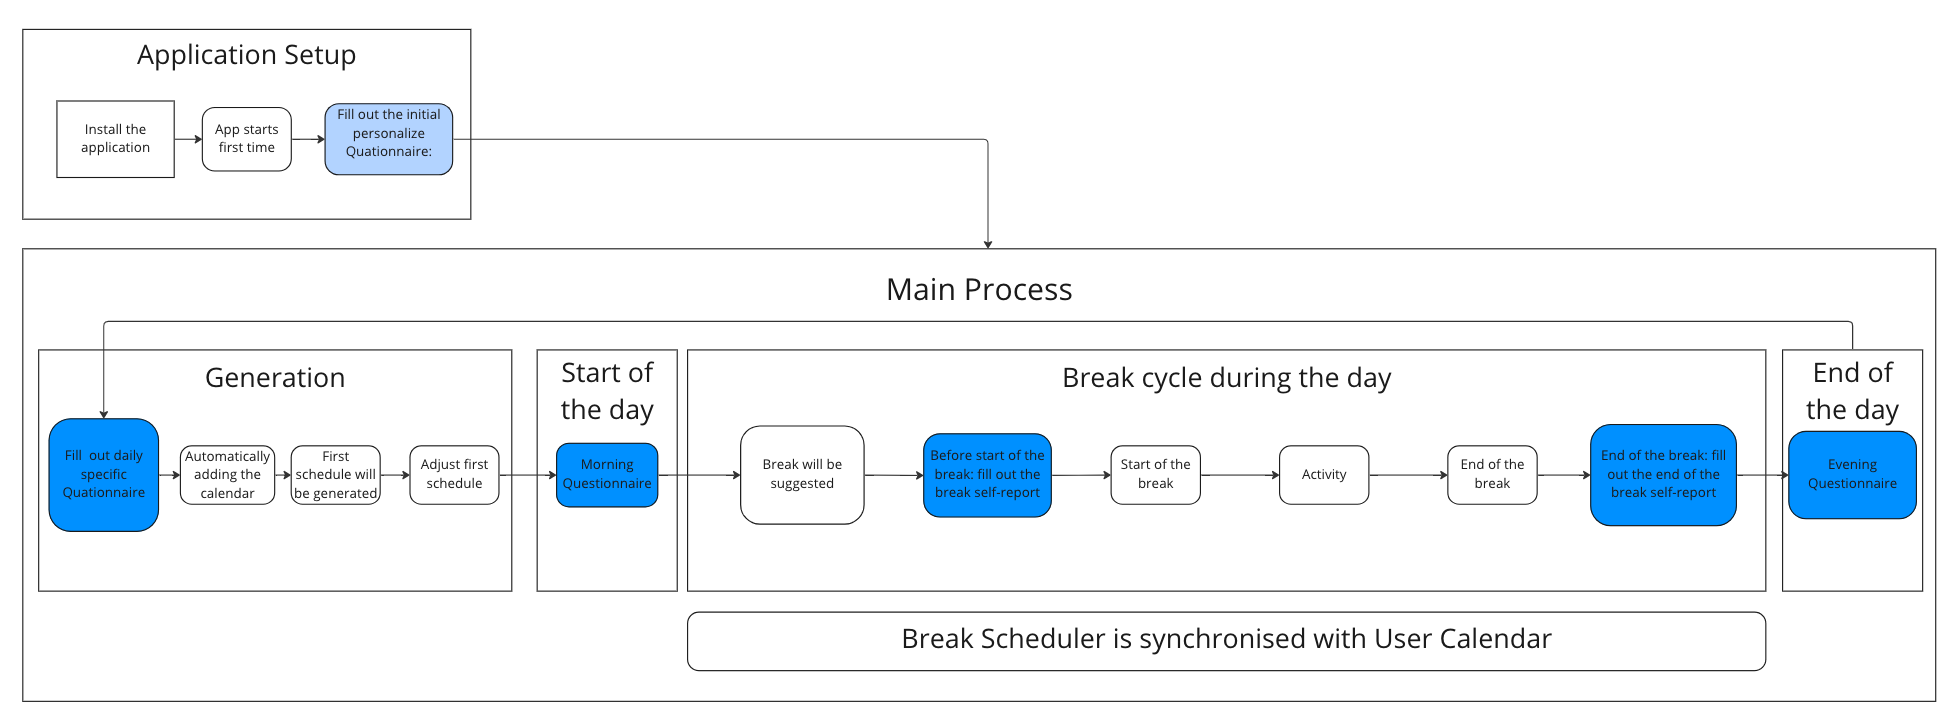
\includegraphics[width=15cm]{hasel_thesis/images/userflow_v2.png}
    \caption{Break Scheduler user flow}
    \label{fig:user-flow}
\end{figure}

As shown in figure \ref{fig:user-flow} the user will initially start with the application setup. At this state, the user will set up the Break Schedule for the first time, so they need to connect their personal calendar and define their break interval and duration. Each user will be asked to select eight activities they want to experiment with. This was defined for the purpose of this study as the usage duration is limited to one to two weeks, and all selected activities need to be tried once to activate the primary value of the rule-based method. The selected activities are the activities which the rule-based system will consider. These are the first personalising steps. Adjusting the break interval and duration enables the user to adjust to their timing preferences, while selecting the activities enables them to adjust to their activity preferences. These values can be adjusted afterwards but not as part of the primary user flow. 


When the first break schedule is complete, the primary user flow will start, with an iteration cycle of one day. Each morning the user will be notified to answer the morning report, which is a short energy report. During the day, the user will also be notified, as shown in \ref{fig:notification}, to take breaks and fill out the before and after break reports, which the rule-based system will use to calculate the experience values. The reminder via notification is an essential factor of the Break Scheduler, as many knowledge workers with high job control struggle to remember to take breaks \cite{McLean.2001}. During the work day, a short notice meeting or a deadline might be approaching, making it essential to reschedule breaks. When working, the user might be on his calendar many times a day. The design choice to enable changes to the break schedule only in the calendar app allows the user to work with his known medium and reduce the application used simultaneously. During the day, the interaction with the Break Scheduler is limited to the notification and the before and after self-reports, which pop up when clicking on the notification. The goal is to minimise the attention needed to interact with the application and minimise the interruption. 

\begin{figure}[htp]
    \centering
    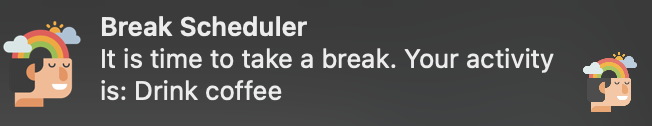
\includegraphics[width=10cm]{hasel_thesis/images/notification.png}
    \caption{Break Scheduler notification}
    \label{fig:notification}
\end{figure}

When it is time to take a break, the Break Scheduler will send a notification which will open the before Break Report. As discussed in the evaluation of the break section \ref{evaluation_break}, it can be challenging to quantify personal resources such as energy, attention capacity or physical well-being. A slider bar for the evaluation was used to give the participant the possibility to make a detailed rating. For simplification reasons, the step points of the slider are 5 points, which makes it easier for the user to rate their resources. For the enjoyability rating of the activity, shown in figure \ref{fig:rating}, an emoticon rating should motivate the user to place a rating.

\begin{figure}[htp]
    \centering
    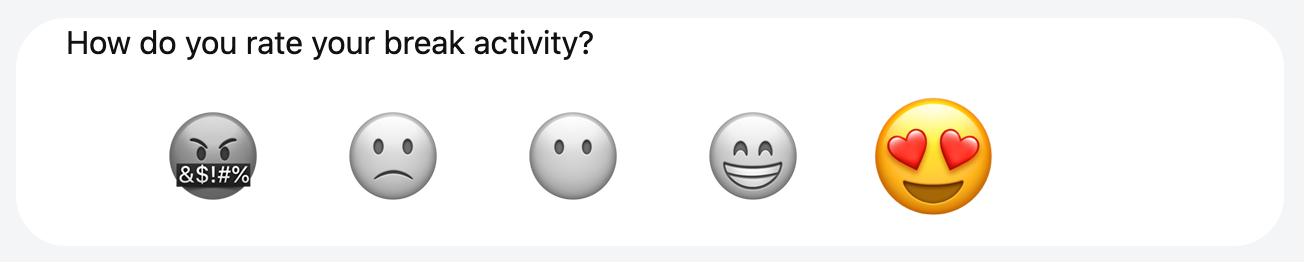
\includegraphics[width=10cm]{hasel_thesis/images/rating.png}
    \caption{Break Scheduler emoticon rating}
    \label{fig:rating}
\end{figure}

During the break, the user should be reminded that they are on a break; therefore, a small window will be opened in the lower right corner, showing the remaining time and the suggested activity. This window is, per design, unmovable, not closable and always in front of everything. The only way to close this window is when ending the break by clicking on the "end break" button. This measure should force the user to take a break and prevent thoughts as "only one last mail", which lead to a switch of task and not taking a break. When the break is ended, the End Break Report will open.

Each evening the user will fill out the evening report, reflecting on the used energy and rating the interval and duration of the breaks. The rule-based system will consider the rating of the break interval and duration before generating the new schedule. More will be explained in the section \ref{rule-based-method-implementation}. Afterwards, the user will be asked for the start and end of their work day and preferred lunch break, ensuring all daily specific inputs are confirmed. Per default, the values of the last time will be shown, enabling users with similar schedules to continue faster. When the schedule for the next day is generated, the daily cycle will start again.

The users are welcome to visit the dashboard or review their activities or reports in between the primary user flow. The user can see all critical information at a glance on the home screen, shown in figure \ref{fig:dashboard}.

\begin{figure}[htp]
    \centering
    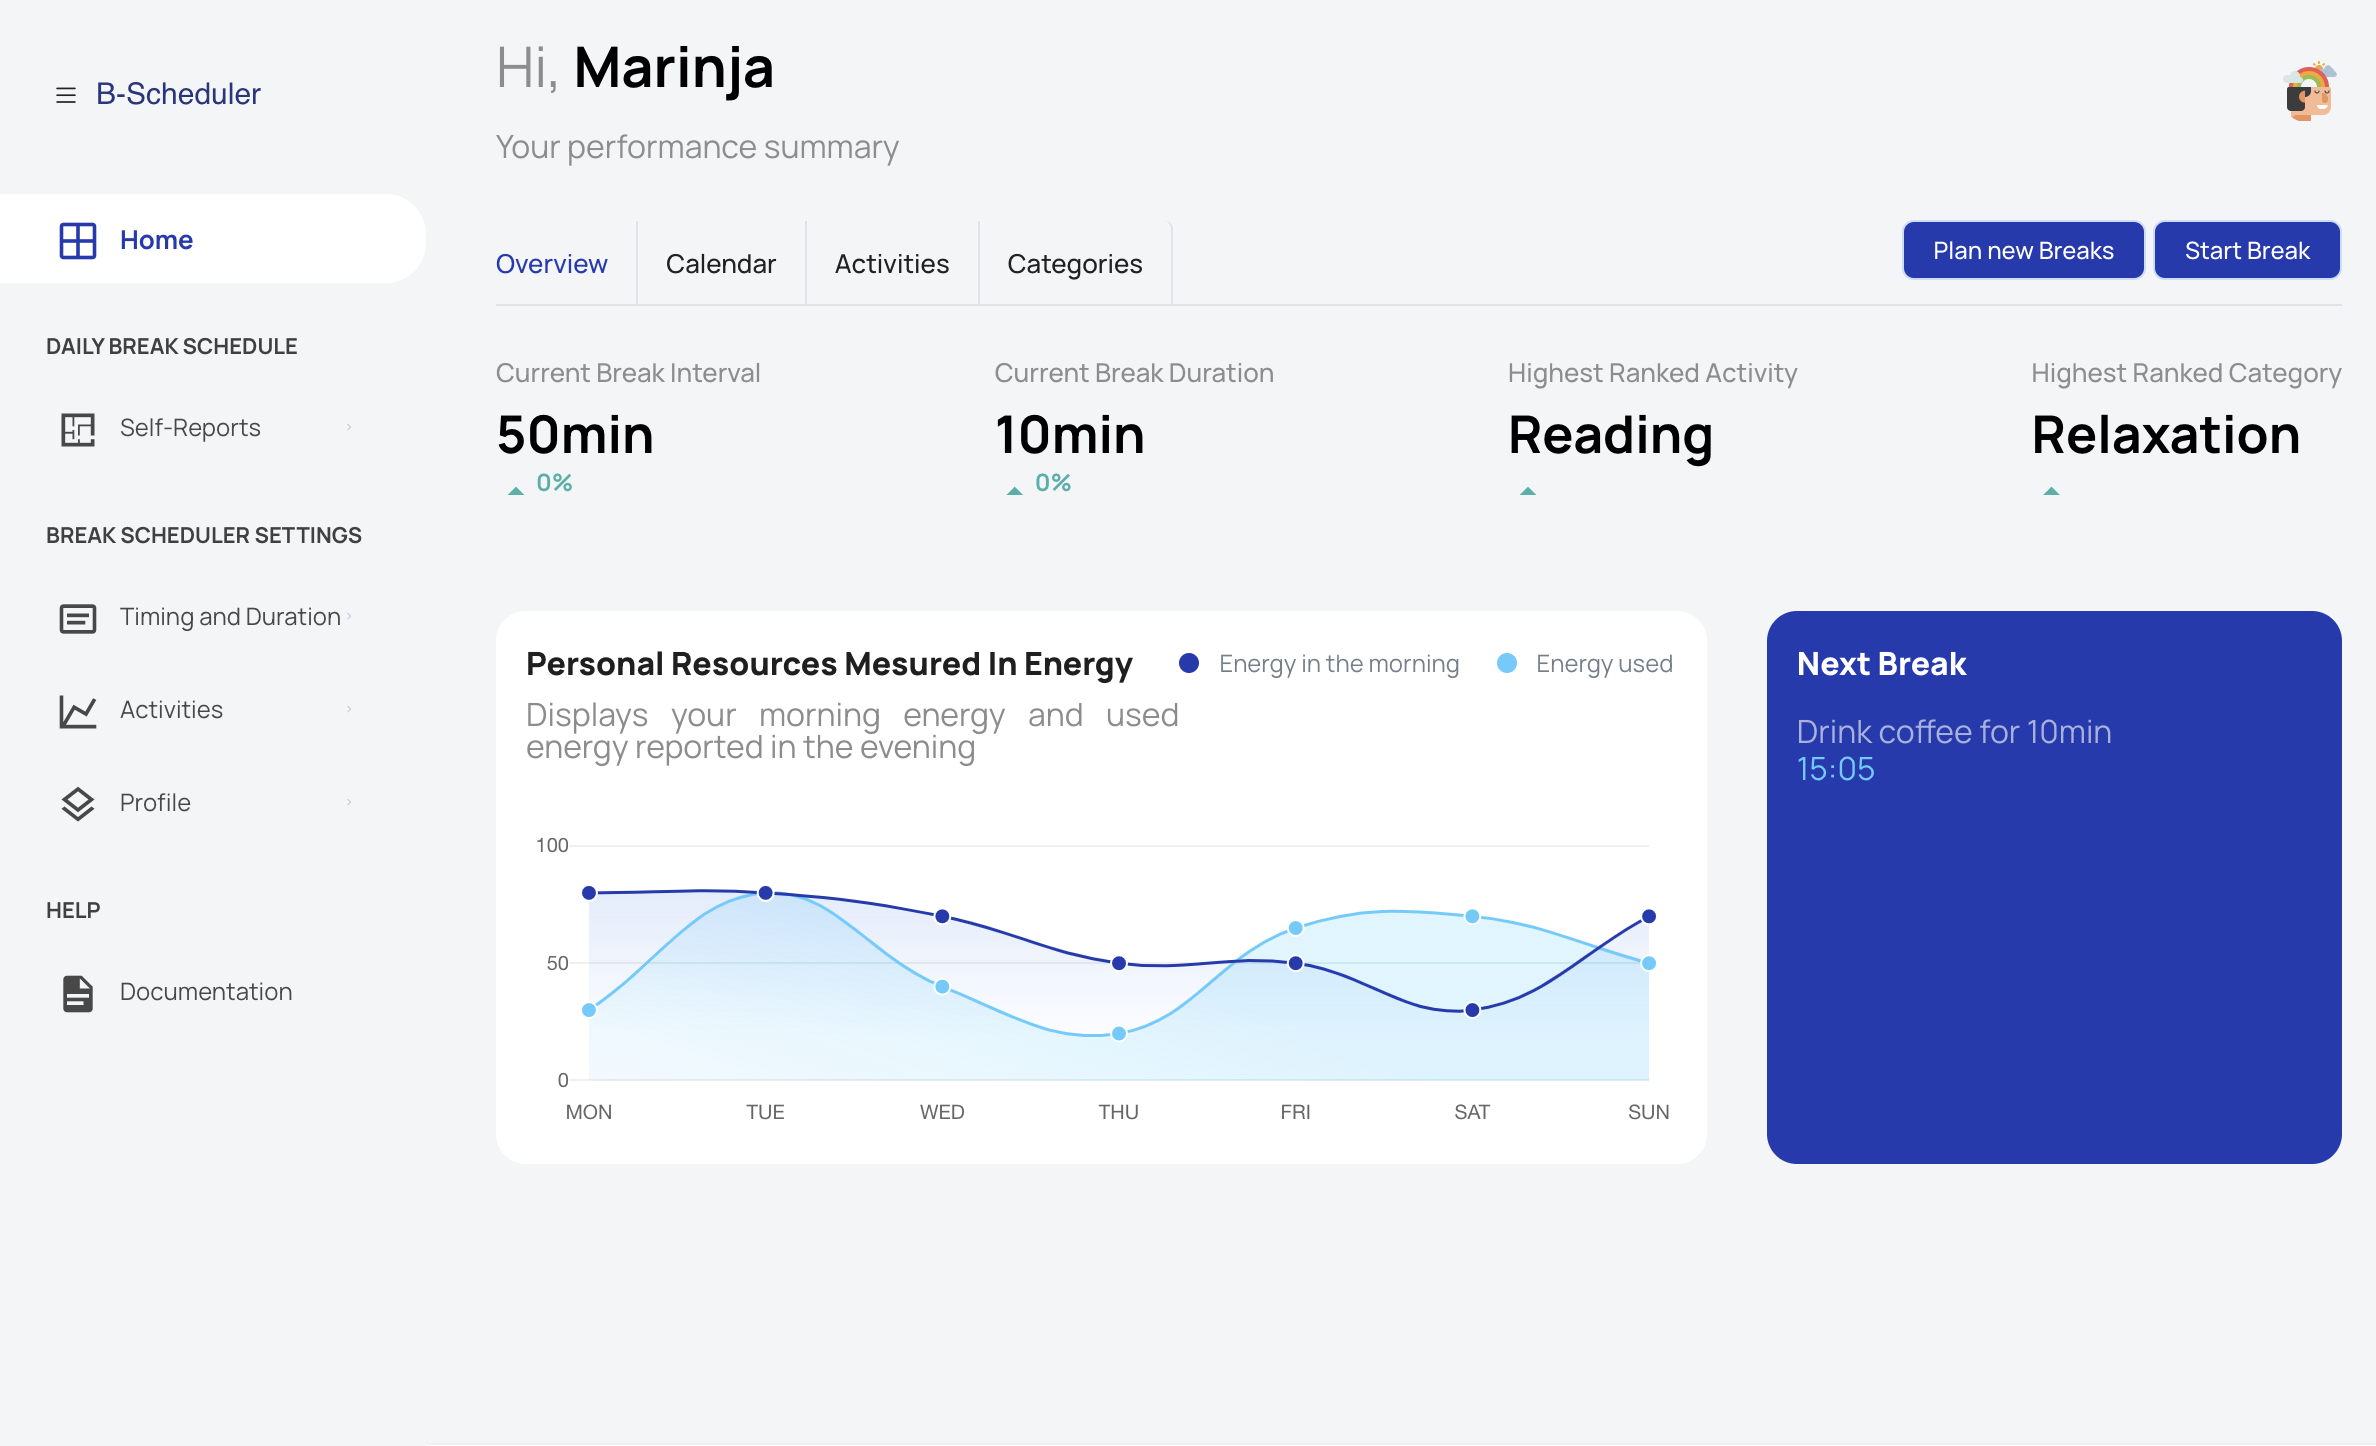
\includegraphics[width=15cm]{hasel_thesis/images/dashboard.png}
    \caption{Break Scheduler landingpage}
    \label{fig:dashboard}
\end{figure}

On the left side, the navigation bar helps the user navigate to all pages. All main pages, such as the calendar, activities or categories, are linked directly in the middle of the page, where the user can easily find them. Two blue buttons, "Start Break" and "Plan new Breaks", are on the same level as the main pages. Therefore, the user can find all main functionalities as well as the navigation to all evaluation pages in the middle of the window, accessible with one click. "Plan new Breaks" is needed when the user did not plan the breaks the evening before, and "Start Break" can be used to start a break, which can also be achieved by clicking on the notification. The overview page displays the current break interval and duration, along with the highest-ranked activities and highest-ranked category. The arrow below these values also indicates whether the values increased or decreased from the last adjustment (e.g. the interval was increased by 30\%). It was a design choice not to incorporate the overall time spent in breaks, as this can lead to an unhealthy feeling towards breaks, as taking a break is still often viewed as unfavourable or "time not spent on productive tasks". As shown in the background section \ref{background}, taking breaks is essential to keep performance high and, therefore, productivity. However, such negative feelings towards breaks could be triggered by showing the overall time spent during breaks.

Another analysis feature displayed is the personal resources chart, which shows the energy rating from the morning report and the energy used from the evening report for each day of the week. This line chart helps users to reflect on their use of personal resources during the week. It should also enable them to find particular patter in their personal resources. For example: If the users use more energy during the day than they have in the morning, the users could get sick after some days as they continuously oversteps their personal boundaries. 

Another important feature on the overview page is the display of when the next break is planned and what the suggested activity is. This essential information is displayed with a bright blue as an eye-catcher. The activity and the category page have a simple yet useful design. All information is shown in a blink of an eye, and possible actions are visualised with familiar icons, such as the delete or edit icons. 

The first draft of the application was tested with a small \textbf{test team} of three people who were using it for multiple days. This test team was not part of the primary evaluation afterwards. The test team used the application during their regular work day, which was an excellent test to evaluate the visibility during working hours. During the test period, the test participants wrote down all bugs or questions they had, which was discussed at the end of the test in a short evaluation discussion. The participation group could find minor bugs which could be resolved for the primary evaluation. Additionally, it became apparent that an onboarding session in which the user will be supported when installing the application and given a short tour of the application decreases the error rate at the beginning. It also helps the users understand the concept more quickly and builds trust, as they know what to do from the start. These onboarding sessions were then integrated into the primary evaluation.


\section{Functionality Design}
\begin{comment} 
Description of the features and functionality of the Personalized Break Scheduler, such as break reminders, break logs, and statistics
Explanation of how these features support the overall design goals and user needs
Discussion of any technical considerations and constraints in the design process


Explanation of the application's core functionality, such as scheduling breaks, integrating with the user's calendar, and storing data
Overview of the technical architecture and how the different components of the application interact and communicate with each other
Discussion of how the functionality supports the user's goals and meets their needs, such as ease of use, accuracy, and data security
Explanation of any features or functionality that have been added or omitted based on user feedback and testing
Discussion of how the functionality has been tested and validated, including any methods used for testing and debugging
\end{comment}
This section will cover the src section of figure \ref{fig:architectur}. This section includes all the main functionalities of the Break Scheduler. All features of the Break Scheduler can be grouped into four groups: personalisation, Rule-Based Method, Calendar Integration and Database.

\subsection{Personalisation} \label{personalization}
Personalization of the Break Schedule is a key factor. All 3 key features of a break: timing, duration and activity need there to be adjustable. That is why the break interval and duration are defined by the user in the setup phase of the application. But also, afterwards, the user needs to be able to adjust these values. Different features of the Break Scheduler enable the user to adjust interval and duration to their needs.

One way to adjust the interval and duration is by the Rule-Based-System at the end of each day, before scheduling the breaks for the next day. This adjustments are only small and in relation to the current time interval, but are part of the main user flow during the day. Further details will be discussed int the section \ref{rule-based-method-implementation}.

\begin{figure}[htp]
    \centering
    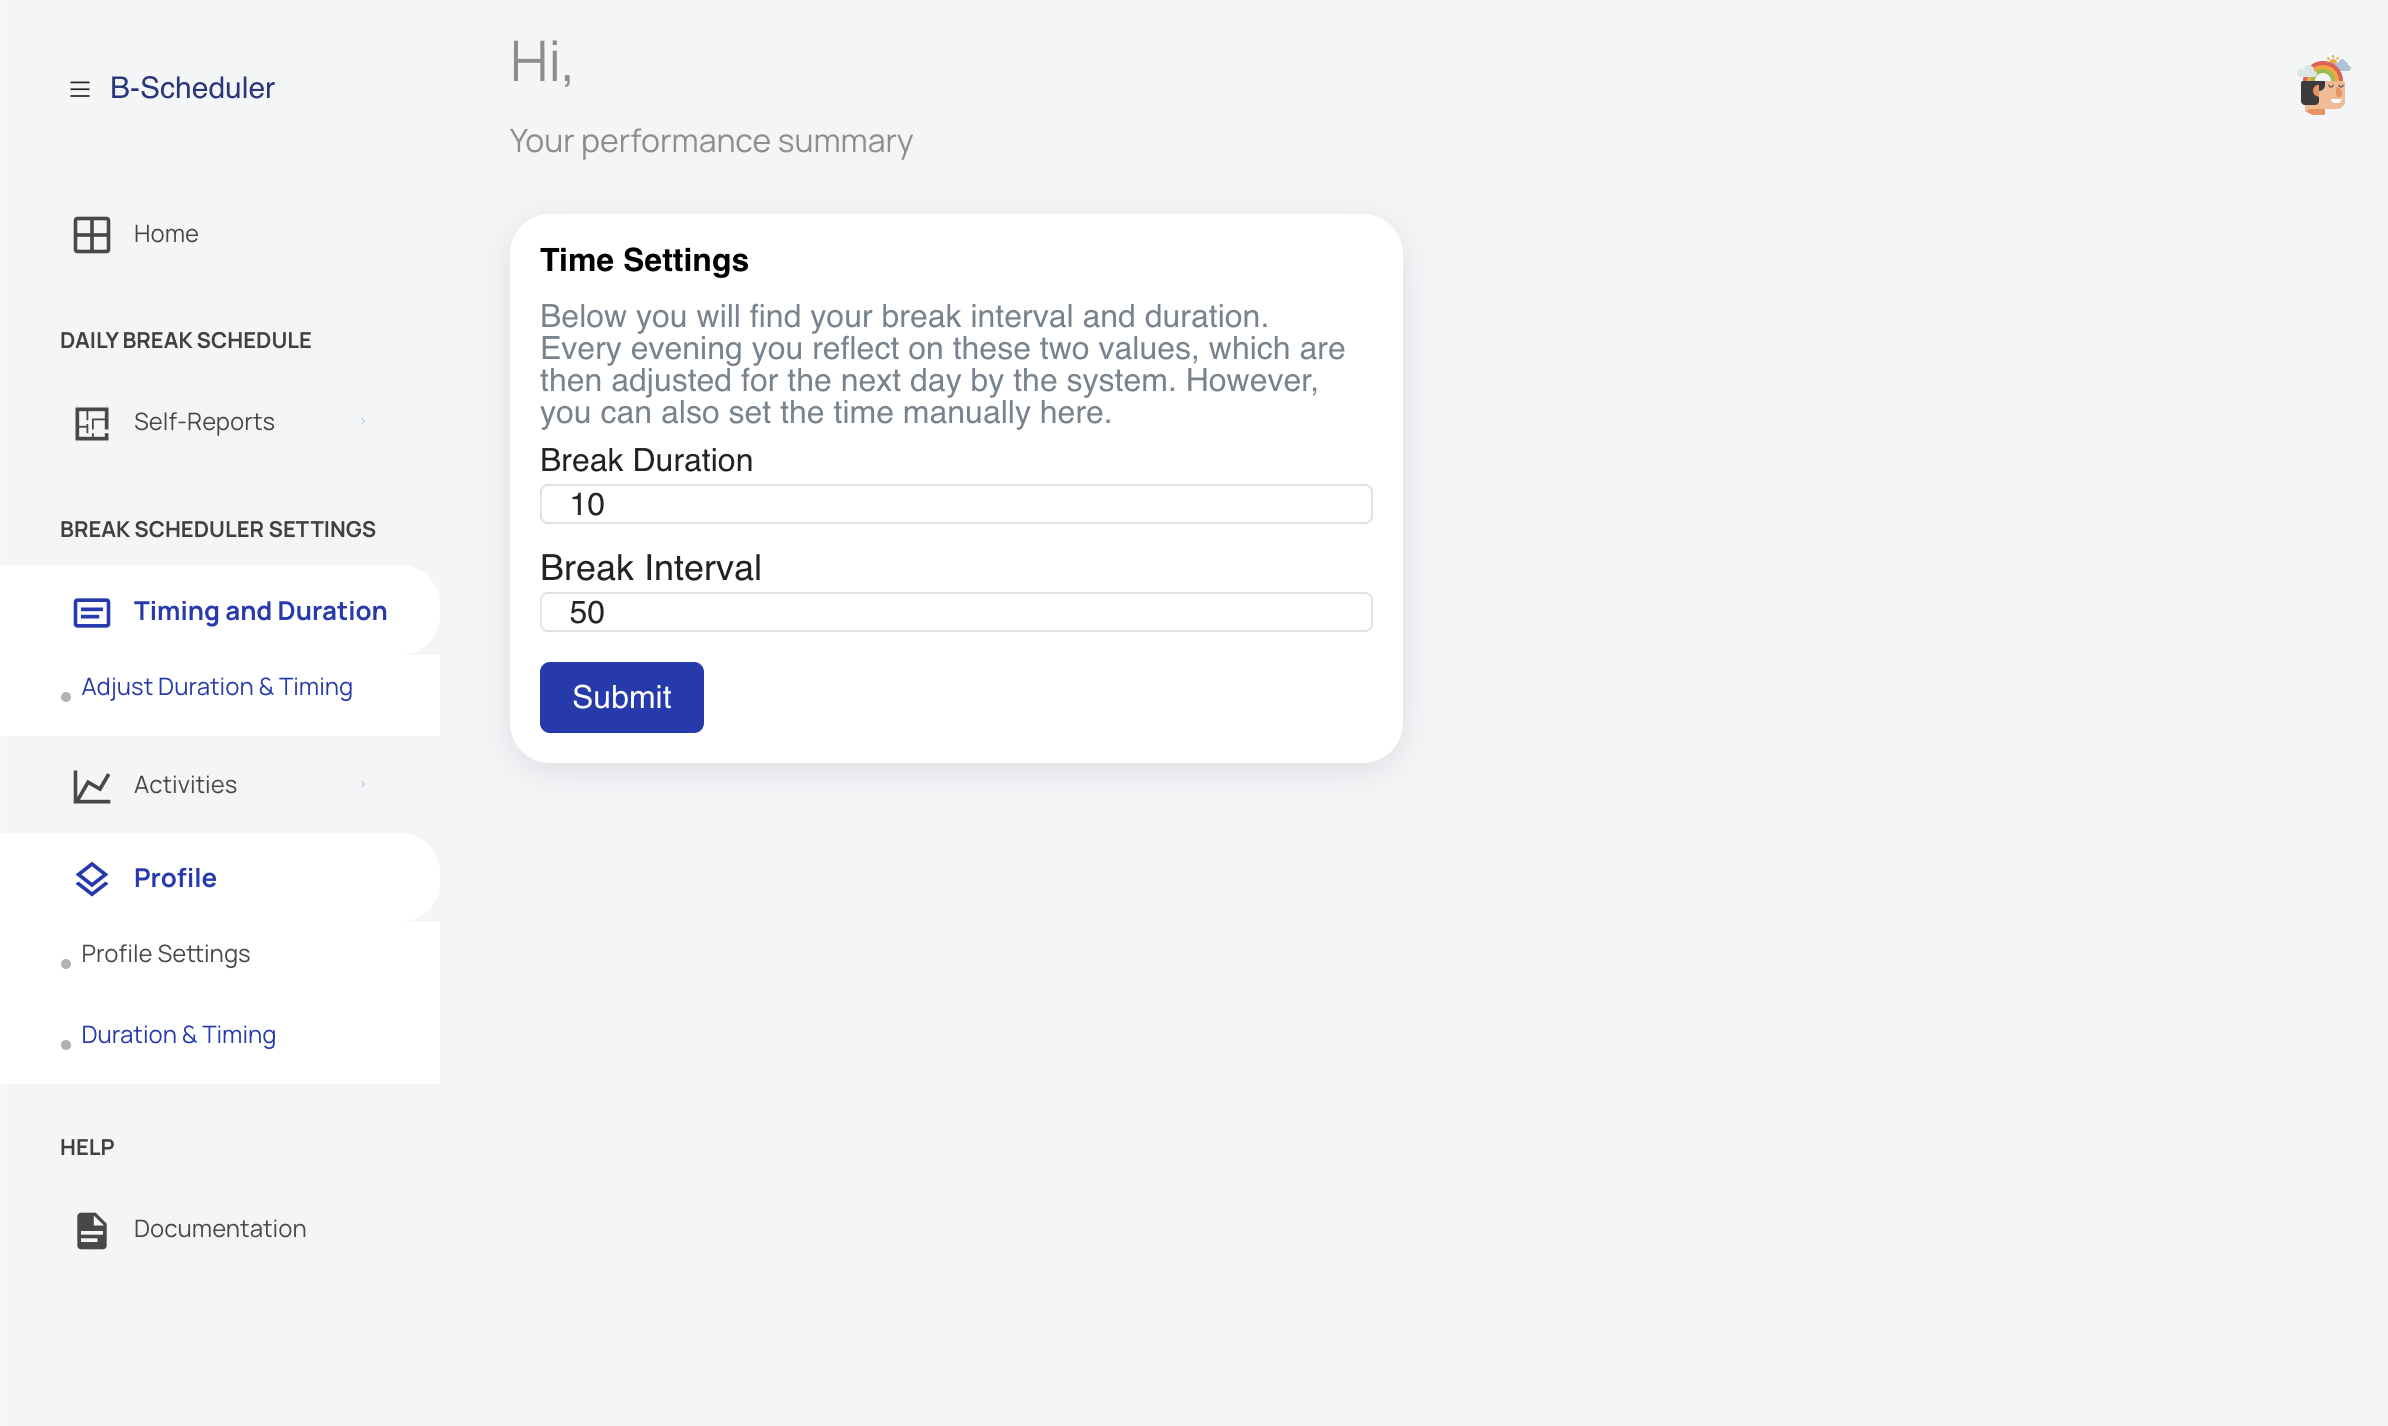
\includegraphics[width=15cm]{hasel_thesis/images/adjust_timing.png}
    \caption{Break Scheduler adjustment of timing and duration}
    \label{fig:adjust_timing}
\end{figure}

Another way to adjust the interval and duration is by hand adjusting Interval and duration. In figure \ref{fig:adjust_timing}, the window to adjust the timing and duration is shown. The new interval and duration will be considered by the next generation of breaks.

As the generated breaks are synchronised with the calendar of the user. The break timing can also be adjusted in the calendar itself, which ensures flexibility during the day, and helps to user to adjust when the planning needs to change. More will be discussed in the \ref{calendar_integration}.


\subsection{Rule-Based Method Implementation} \label{rule-based-method-implementation}

The Rule-Based Method contains three main features: the generation of the breaks, updating of the experience values and adjusting the break interval and duration.

\begin{figure}[htp]
    \centering
    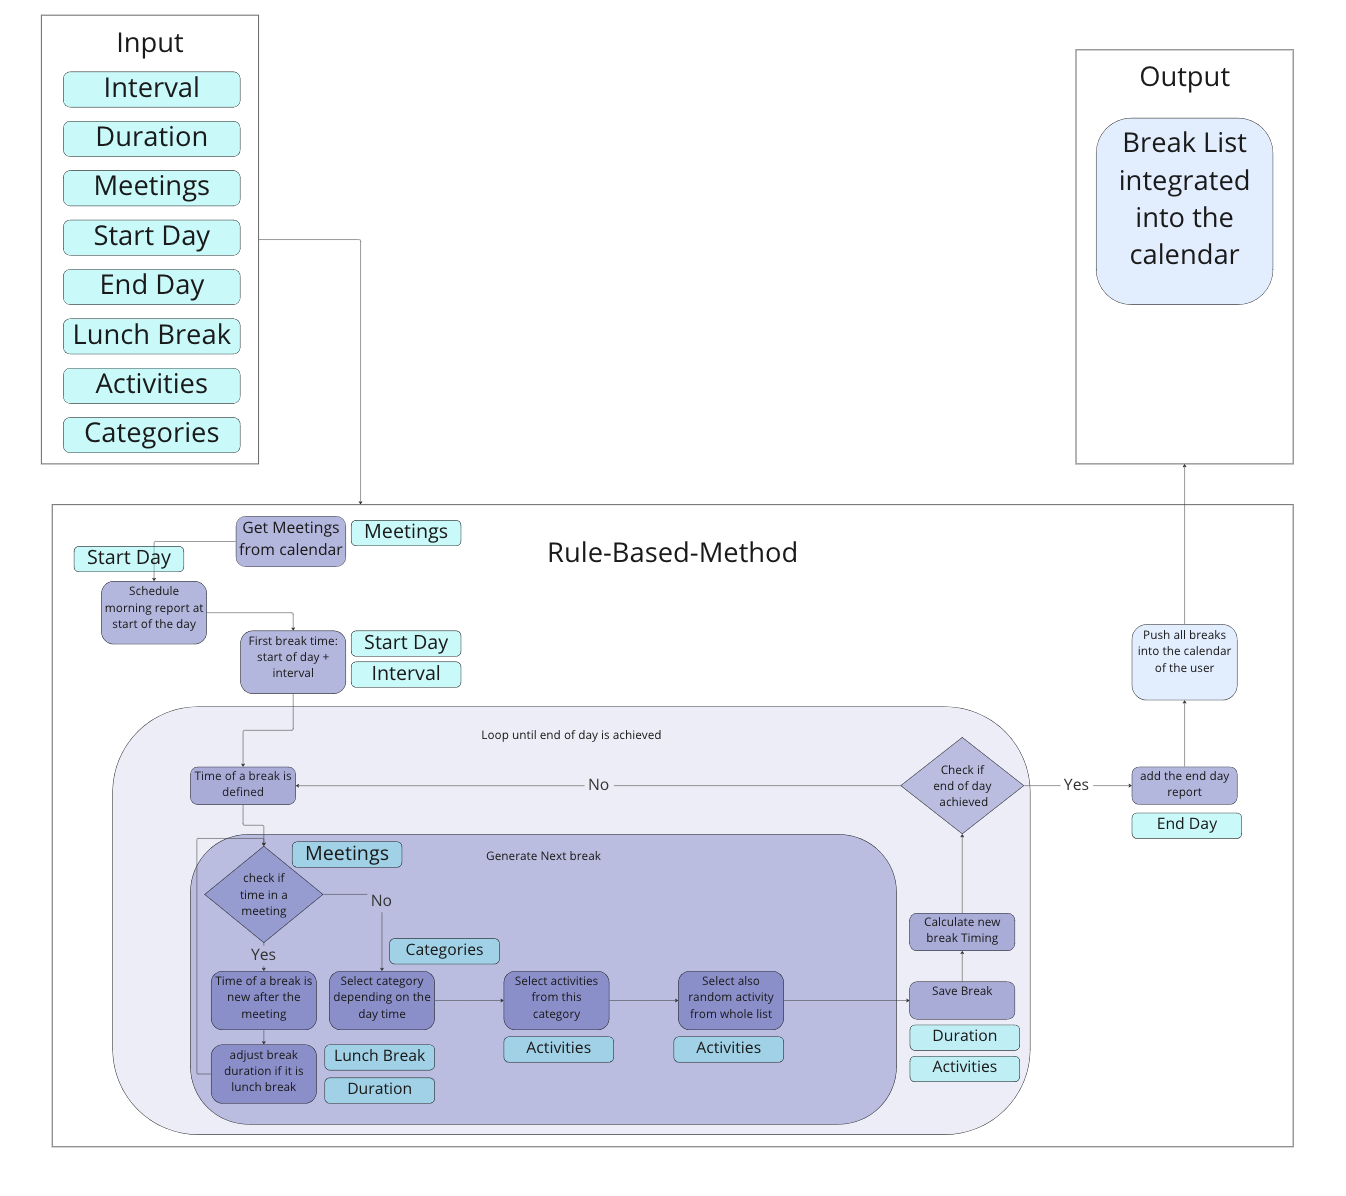
\includegraphics[width=15cm]{hasel_thesis/images/rule-based_method.png}
    \caption{Rule-Based Method Process}
    \label{fig:rule-based_method}
\end{figure}
\textbf{Generation of Breaks.} For the generation of breaks, in figure \ref{fig:rule-based_method} the process of the rule-based system is visualised. As input, the method needs the interval and duration, activities and categories which are saved by the application. The user needs to enter the specific start and end of the day as well as the lunch break duration. The meeting for the selected day will be automatically gathered by the application. When all the input is available, the system will start by saving the morning report at the start of the day. After that, the first break start time is defined as the start of the day plus the interval. Now the method first checks whether the timing with the break duration is in a meeting. If so, it reschedules the timing after the meeting, updates the break duration, as it could already be lunchtime, and checks again if the break is in a meeting or not. If the planned break is not in a meeting, the activity will be selected. Each activity has a minimum and maximum duration, as well as an experience value. The minimum and maximum duration is used when selecting an activity for a certain break duration, as it is for example, impossible to make outdoor training in a 5min break. The category also has an overall experience value but also a morning, lunch and evening experience value. This helps us with the selection of the category depending on the daytime. Before the activity is selected by the rule-based method, the category with the highest experience value for this daytime will be selected. Afterwards, the activity from this category with the highest experience value, which fits the given duration, will be selected. However, as long as there is a category or activity that was not yet tried out, this will be selected. When the activity is selected, one random activity out of the whole list will be selected. This random activity should add some randomness to the process and reduce possible bias from the rule-based system. When the suggested and the random activities have been selected, the break with timing, duration, suggested, and random activity will be saved, and it will be checked whether the end of the day is already achieved. During the last interval of the day, there are no breaks scheduled to enable the user to finalize his work. When the last interval of the day is already achieved, a short break for the evening report will be scheduled. All scheduled breaks will be saved in the database, but also and most importantly all breaks will be scheduled in the calendar of the user. The process is finished when the user can see all breaks in his personal calendar or in the calendar window in the application.

\textbf{Update the Experience Values.} Before and after each break the user will fill out a short self-report, which asks for the selected activity and about the current state of their energy (e), attention level (a) and physical well-being (p). After the break the user also rates the activity (r). In order to calculate the experience value, the rule-based system calculates the following:

$$ rawExpValue = \frac{e_1- e_0}{10} + \frac{a_1- a_0}{10} + \frac{p_1-p_0}{10} + \frac{r}{10} -5$$

$$ expValue = Round(rawExpValue/5)*5$$

As e, a, p and r are values between 0-100, the difference will be divided by 10. As the r value should also be negative if the activity was not perceived, 5 will be substrate. Therefore the value r can go from -5 to 5. The rawExpValue is raw expectation value, which needs to be rounded to the next number that is divisible by 5, in order to group more activity together when selecting the activity with the highest experience value. This value will be added to the experience value of the activity, and also to the overall and daily specific experience value of all related categories of the selected activity.

\textbf{Update Break Interval and Duration.} Each evening the user will be asked to fill out the evening report where they rate their used energy as well as the break interval and break duration. The user can select whether the interval was good, too long or too short, the same holds for the break duration. According to the user input the following calculation will be done:

"Too Short" for interval (i): $ i = i + Round(i/10) $

"Too Long" for interval (i): $ i = i - Round(i/10) $

"Too Short" for duration (d): $ d = d + Round(d/3) $

"Too Long" for duration (d): $ d = d - Round(d/3) $

This simple calculation was chosen in order to ensure a relative change, and helps the user to find a specific target time, as the both values can step by step level off to the target time. The chosen relative change is higher (1/3 instead of 1/10)  than the interval, as the duration values is normally smaller and the same relative change (1/10) would not really have a impact on the break duration: e.g 10min break duration would be 11min if the duration was too short. With the higher relative change the new duration is 15min. This new interval and duration will than be used to create the new Breaks.


\subsection{Calendar Integration} \label{calendar_integration}

In order to integrate the calendar into the Break Scheduler two APIs were used: Google API and MS Graph API. Both APIs ensure the automatic synchronisation between the Break Schedule and the personal calendar of the user. 

\textbf{Google API.} Google provides a API to connect their Google calendar using their OAuth2 Client API. For a new Client needed to be opened in the google cloud. As the Break Scheduler is still in the test phase, the user needed to be entered manually into the google client, enabling them to connect the Break Scheduler with the Google Calendar. When selecting the google Calendar, the user will be redirected to the Google login screen, where they can login and give the application permission to read and adjust calendar data. The API will generate a token which will be saved by the Break Scheduler, ensuring that the user only needs to login once.

\textbf{MS Graph API.} Similar to the google API, the first step to use the MS Graph API is to register an app in the Azure directory. When a user selects the Microsoft Calendar, they will be redirected to the Microsoft login page, were they can login and give the app the permission to read and change calendar data. The API gives back a token which is saved by the Break Scheduler. In contrast to the Google API the user need to login each time the application is started new.

Each minute the Break Scheduler will send a request to the API and updates the breaks and meeting data of the user, in order to adjust to changes during the day. The notification send by the Break Scheduler will be adjusted accordingly.

\subsection{Database} \label{database}
As already described, the database is a simple SQLite database, which is suitable due to the fact that all information is saved locally on the users machine, which reduces data privacy issues. The database considers of different tables as shown in figure .........

-------------------- add DB visualisation  -----------------------

The tables Activity, Category, and Settings are actively used by the Break Scheduler to generate the new Breaks, while the table for the Break reports and the Morning and Evening reports are stored to show them to the user. The Logs and the Break table are currently only used for analysis purposes for the User study.


\begin{comment}

morning and evening report
Each morning the user will be asked to rate their current energy rate, which will be a measure of the personal resources available for the rest of the day.  At the end of the day, each user will be asked how much energy he used during this day, which should be a measure to visualise the used personal resources. The term energy was used instead of personal resources as many users find it difficult to rate their personal resources and easier to rate their current energy on a scale from 0 to 100. These morning and evening reflections should enable users to find specific patterns between their resources and well-being. For example: If you use more energy during the day than in the morning, you could get sick after some days as you continuously overstep your personal boundaries. This data is additional self-reflection material which is not yet included in the rule-based system of the break scheduler but will be shown in the dashboard of the tool to enable the user to overview their personal resources and used resources during the day.


In addition to the used energy, the evening report will also ask about the break duration and the break interval. For both, the break duration and the break interval, the user has three selections each: Good, too long or too short. When a break duration or interval got the rating "good", the time will not change. If it was too long or too short the time will be adjusted by a percentage of the existing time. More is explained in the implementation of the rule-based system.





As the goal of this thesis is to raise awareness of their break habits as well as enable the user to find beneficial activities, the solution uses self-reported input data. 
The goal of this work is to develop a personalized break planner that supports users in finding the opportune time with a focus on the activities, to develop good/effective break habits. The emphasis is to support the user in analysing his break preferences and not on dictating the "best schedule" and should leave room for flexibility during the day.



%Nun sollte ein (separates) Implementation-Kapitel folgen (ich glaube das hast du in 4.0.1 vorgesehen). Hier kannst du beschreiben, wie du die Key-Konzepte effektiv implementiert hast.
\textcolor{red}{all not yet finished an don't know what to say here}
- Overview of the Break Scheduler software
- Description of the software's features and functionalities
- Explanation of the software's design and development process

For the implementation of the Break Planner, it was important that it will run on the user's laptop and that all data can be saved locally on the laptop itself, so only the user has full control over their data and data privacy issues can reduce. In order to realise the Break Planner, a Desktop application was preferred that is able to run on different operating systems without a lot of extra effort. Therefore an Electron app was built using typescript. The database of the Break Scheduler is a simple sqlite3 database which will constantly be updated during the use of the application. 


    

\section{Procedure}
One of the first steps before starting with the implementation was to define the concept of the Break Planner. Supporting the definition of the goals of this tool, the first step was to define the main objectives. During the related work phase, it becomes apparent, that there are a lot of studies focusing on the break time and the duration, but only a few studies are looking at the break activity. Additionally,  whereas there are a lot of different tools to plan static breaks which only consider the timing and duration, no tool could be found, which helps a user to find good breaks beneficial to their energy, attention and physical well-being. Therefore the following 3 Key objectives were defined for the Break Planner:

•	Improve awareness of users on their existing break habits and their effectiveness
•	Enable users to self-reflect on their personal resources, such as attention, energy and physical well-being.
•	Empower users to identify good break activities that restore their personal resources

After the high-level concept was done, the requirements were defined and the customer flow was analyzed (Add pictures here).


\end{comment}


\chapter{Methodology}
%Dann folgt ein Preliminary Evaluation Chapter: hier beschreibst du zunächst die Methode und anschliessend Resultate
This chapter describes the method and procedure used in this user study to answer the effectiveness of the Break Scheduler application in raising awareness of personal resources and enabling users to learn more about their break habits. This section provides a detailed explanation of the sample selection, study design, data collection procedures, and data analysis methods used to answer the research questions stated in the introduction, enabling the reader to reproduce the experiments when needed. The following subchapters provide more information on each aspect of the methodology.

\section{Participants}
\begin{comment} 
- Description of the sample size, criteria for inclusion/exclusion, and demographics of the participants

From pre-Q:
- 50% male, 50% women
- most of them are in a relationship with no kids
- most of them would say, they are introverted people ( 8 vs. 5)
- highest education degree is a bachelor's with also many with master's or people who are currently in their bachelor's or further education degree
- most of them work most of their work day on the laptop
- 0 of them have a normal workload, vs 5 which have a high demand and 1 which has a low work demand
- most of them have a high job control and can therefore choose their own time planning
- and most of them can choose their work location most of the time or sometimes
- their work environments are open mined concerning breaks at the workplace
\end{comment}
 The study includes a sample of 13 knowledge workers with different backgrounds (students and employees) working in various industries, ranging from IT, chemistry, and mathematics to education, aged 20-40, living and working in the German-speaking part of Switzerland. The recruiting was done by word-of-mouth approach. Each participant was asked to participate with their main work laptop/computer as the application needed to be incorporated into their daily work. As the Break Scheduler is a desktop application, the participants needed to be able to install this application on their device, which already pre-eliminated people who were not allowed by their employers to download specific applications on their work machines. Within this sample group, all three main operating systems ( macOS, Windows and Linux) were represented, eliminating the exclusion risks of certain groups of knowledge workers.

\section{Study Design}
\begin{comment} 
- Explanation of the experimental design, including control and intervention groups, pre- and post-tests, and other relevant details
\end{comment}

This experimental study tests the Break Scheduler application for its effectiveness. To achieve this, the control conditions of each participant were gathered by a pre-intervention Questionnaire, which asked about demographic data as well as their awareness regarding their personal resources and daily break habits. This with-in-study design ensures each user acts as their own control, enabling a pre-and post-intervention evaluation to answer the research questions. The selection of participants was done by a word-of-mouth approach in combination with a snowball sampling method and eliminated participants who could not install the application on their work machine. The participants in this study were voluntary and could be stopped at any time. Other than insights into their results, no monetary or non-cash deposit was offered.

This study conducts three phases: Pre-Intervention, Intervention and Post-Intervention phase. 

The Pre-Intervention phase provides insights into the participant's demographical data and their awareness of their personal resources and break habits. These phases refer to the control conditions to define the pre-intervention state of each participant. The participants are asked to complete the \textbf{pre-questionnaire} in the form of an online survey with questions about their existing break habits and awareness of personal resources. This questionnaire should represent the baseline of the user's awareness of personal resources and break habits with the influence of the Break Scheduler. The survey also includes demographic questions (e.g., age, gender, occupation, work background) to control for potential confounding variables. This pre-intervention questionnaire is attached to this thesis.

After completing the pre-intervention questionnaire, the intervention phases start, where the researcher will guide the participants through installing the \textbf{break scheduler application}. Subsequently, they will be asked to use the break scheduler for five consecutive workdays during their regular work. The break scheduler app includes one morning and evening self-reflection questionnaire and a short pre-and post-break self-reflection questionnaire. Some self-reflections are part of the application, while others are used to collect qualitative data for the preliminary user evaluation. All collected data is stored in the app's local database. All data produced during the intervention will only be stored locally on the user's machine and can only be accessed by them. However, as part of the consent form, all participants will sign that they will grant access to their database file after the intervention for study purposes.

After completing the intervention phase, participants will be asked to answer the \textbf{post-questionnaire}, where they are asked about their experience with the break scheduler app, their learning, and potential ideas for improvements. They are also asked about the advantages and disadvantages of the implementation. In this post-intervention state, participants will rate their awareness of their resources and break habits again and will rate the impact of the Break Scheduler.

The pre-and post-intervention will be compared in an evaluation analysis to answer the research question.


\section{Procedure}
\begin{comment} 
- Step-by-step description of the procedure followed in conducting the study, including data collection, administration of the recharge breaks, and any other relevant details
\end{comment}
To enable the reader to replicate the conducted results, all step-by-step tasks are stated and further elaborated.

\textbf{Participants:} Participants were recruited through a word-of-mouth approach and a snowball sampling method by asking friends and acquaintances if they would be willing to participate in the study. A total of 18 knowledge workers agreed to participate. Out of these 18, two participants were used in a pre-evaluation testing phase which eliminated them from participating in the study. Four of them needed to cancel the study during the intervention phase due to personal reasons. It led to a total of 12 participants fulfilling all three mandatory stages.

-------------------- add diagram of user demographics ----------------------

\textbf{Pre-Questionnaire:} Before the intervention, all participants were sent an online survey to collect demographic data and information about their awareness of their personal resources and break habits. This study was filled out before the intervention started. All detailed questions of the Pre-Questionnaire can be found in the appendix.

\textbf{Onboarding:} At the start of the Intervention phase, a short onboarding session was held with each participant to install the Break Scheduler application and provide a brief introduction to its use. Participants were shown how to connect the Break Scheduler with the calendar for synchronisation and how to fill out the different self-reports and the applications' main features.

\textbf{Intervention:} Participants were asked to use the Break Scheduler application for a period of one to two weeks, during which time they were encouraged to log their personal resources with a morning and evening report as well as their break activity and their well-being before and after the break measured in an energy, attention capacity and physical well-being rating. They were also asked to rate the activity after each break. Each evening when filling out the evening report, the participant uses the application to schedule breaks for the new day. Participants were able to contact the researcher if they had any questions or problems with the application.

\textbf{Post-Questionnaire:} After the intervention phase, participants completed a post-questionnaire that included questions about their awareness level after the intervention, as well as the impact of the Break Scheduler and their implementation of the tool. All detailed questions of the Post-Questionnaire can be found in the appendix.

\section{Data Analysis}
\begin{comment} 
- Explanation of the statistical methods used to analyze the data, including descriptive statistics, inferential statistics, and any other relevant techniques

The data analysis section of your study is where you describe the methods you used to analyze the data you collected. This section should include the following elements:

Data Cleaning: Describe any steps you took to clean the data, such as removing missing values, checking for outliers, or transforming variables.

Descriptive Statistics: Provide summary statistics for the demographic and pre- and post-intervention data, including means, standard deviations, frequencies, and ranges.

Inferential Statistics: Describe the inferential statistical methods you used to analyze the data and test your hypotheses. For example, if you were comparing the mean level of personal resource recharge between the intervention and control groups, you might use a paired t-test or a repeated measures ANOVA.

Results: Present the results of your statistical analysis in a clear and concise manner, including tables, figures, and effect sizes. Interpret the results in the context of your study, including any significant findings and their implications.

Limitations: Discuss any limitations or limitations of your study, including sources of bias, limitations of the data, or limitations of the statistical methods used.

Conclusion: Summarize the main findings of the study and provide implications for future research.

This section should be written in a clear, concise manner that is accessible to readers who may not have a strong background in statistics. Any statistical tests should be accompanied by an explanation of the test and its assumptions, as well as the results of the test and their implications.
\end{comment}
\textcolor{red}{data analysis not finished}

5.	Measurements:
5.1.	Quantitative Data Collection:
Rule-based System:
The rule bases system's values (e.g., experience values, break interval and duration, etc.) will be saved in the Database file. This file will be manually sent back to us by the user for this study. These values will indicate which activities and categories will be ranked best. These activities and categories can be compared to the qualitative data the user is providing. 
Report files:
From all the reports (e.g., morning and evening reports, as well as before and after break reports) saved in the database, we know how many reports were filled out per day, indicating how actively a user used the tool and how many daily breaks they did. This number can be compared with the number of the pre-intervention questionnaire. 
Settings:
During the break schedule, the user will experiment with their break interval and duration and eventually find their preferred duration and interval timing. It will be interesting to compare the numbers of the break schedule with their guessed break interval and break duration in the pre-intervention. These numbers can also vary from person to person.

5.2.	Qualitative Data Collected
Daily Self-Reflections
Daily self-reflection should help the user to reflect on their day and compare their energy level to their used energy during the day. Each person has a limited amount of personal resources which will be used during the day (e.g. resources for attention, decision making or just social interactions). These morning and evening reflections should enable users to find specific patterns between their resources and well-being. For example: If you use more energy during the day than in the morning, you could get sick after some days as you continuously overstep your personal boundaries. This data is additional self-reflection material which is not yet included in the rule-based system of the break scheduler. The user quantifies their energy level in the morning and activities during the day (rating 0-100). The energy minus the activity value will show the difference and help users better understand and manage their personal resources. There are also free text boxes where the user can enter notes about their mental or physical well-being which should help them self-reflect more in-depth and give more insight into their day. This also helps to detect patterns for triggers for physical complaints, for example, headaches. This data will be visualized on the overview page for the user to understand their energy household better. Additionally, it will be used in this study to see if there is any energy change during the week. In the best case, the morning energy will rise, and the used energy will be smaller, which means the user has increased his personal resource and decreased the usage during the day. 
On the other hand, two questions in the evening report reflect on the break interval and the duration. The user can select between the ratings "good", "too long", and "too short". This rating will adjust the break interval and duration for the following break schedule.

Pre/Post-Break Self-Reflections
These short self-reflections should rate the break and are used by the rule-based system to determine the suggested activity. In the pre-break reflection, the user is asked about their energy, attention level, and physical well-being. The same three questions and an overall emoticon rating about the break activity will be shown in the post-break self-reflection. If the difference in the energy, attention and physical level is positive, the break can be considered "good" (resources are recharged). If the difference is negative, personal resources are drained, which is why this break is not considered a "good" one. These values will be added to the sum of the experience value of each activity and the respective categories of the activity. The categories and activities with the highest experience values will be selected for the next generation of the break schedule. In addition to the suggested activities, the break schedule also selects a random activity. Which activity is selected gives exciting insights for the user study and ensures that low-ranked activities can be chosen again and achieve higher experience values. The user quantities their energy, attention and physical well-being before and after the break (rating 0-100). The difference between the after and before will rate whether it was a "good" are a "bad" break.
Additionally, the activity will be rated by an emoticon rating, quantified (-5 to 5) and used by the rule-based system to quantify the break activity. There are also free text boxes where the user can enter notes about their mental or physical well-being which should help them self-reflect more in-depth and raise awareness about their well-being. This data is not used by the break scheduler and is only for self-reflection purposes.

Pre-Intervention questionnaire ()
In the Pre-Intervention Questionnaire, it is crucial to understand the demographical background of the user and their usual break habits. This data is needed to compare their break habits, including the break scheduler and to control for potential confounding variables. Below is a summary of the chapters, and the entire questionnaire is attached.
1.	Demographical data
2.	Awareness of personal resources
3.	Break habits
The questionnaire can be found at the end of this thesis.

Post-Intervention Questionnaire (no content yet, TBD)
The post-intervention questionnaire will give additional information to answer the RQs regarding the impact and the tool. The questions are categorized according to the three RQs : 
1.	Awareness
2.	Impact
3.	Tool
The questionnaire can be found at the end of this thesis.

	
Analysis
A lot of the analysis will be done by comparing the pre-and post-intervention questionnaires. For example, their awareness will be compared to the awareness at the end of the study. Additional qualitative data can enhance the user's answers as to which activity or break interval was preferred the most. In the best case, a correlation can be found between the energy during the day and the ratings of the breaks. 
 
Limitations 
This study has several potential limitations, including self-reflection bias (since participants will be completing the survey and reporting their own personal and physical resources and maybe want to present themselves better for the study) and selection bias due to the self-selection and word-to-mouth approach of the researcher. Additionally, the sample size is too small to make a conclusive statement for a wider group of people. However, some trends can give insight.

\chapter{Results}
\begin{comment} 
Summary of the findings from the study, including any significant effects of the recharge breaks on personal resource recharge
\end{comment}
In the following section, the results of the user study will be presented, including the pre and post-questionnaire as well as the database file information during the intervention week.
\section{Overview of captured Break and Personal Resources Data}


\section{Self-reporting personal resources}
\begin{comment} 
Self-reporting personal resources multiple times a day creates more awareness, helps to be more mindful about how to spend the limited personal resources and helps the user to find beneficial break activities (RQ1, RQ2, RQ3)
\end{comment}
The reporting of personal resources can be split into two subchapters: awareness of personal resources, which includes mainly the morning and evening reports and the awareness of beneficial breaks, which consists of the before and after break reports during the day.

\textbf{Awareness Personal Resources.}
From the Pre-Questionnaire, it could be pointed out that most participants rarely reflect on their resources or only when they are low or in a deficit.  It can be stated that the participants reflect on their personal resources every other day (5x) or barely (4x), and only a few reflect on them every day (2x) or multiple times per day (3x).  Additionally, most of them (12x) do not use a tool to reflect on the resources, only one uses an app, and one uses an activity tracker.  Most of the participants (9x) only reflect on their resources when they are low or they have a resource deficit, as underlined in the following statement of one of the participants: "If they are either really low or really high, then I am more aware of it.  If "normal", then I do not think about it." -[S06]. During the day, most users are not aware of their personal resources.  Some of them, however, reflect on their resources in the evening: "I'm generally aware of a lack of personal resources at the end of a given day.  During the day, I'm very unaware of my personal resources"-[S11].  Also, external factors such as social contact (3x) or high work demand (3x), can motivate the reflection on personal resources: "On days or during weeks where a lot of work has to be done, I am very aware of my personal resources and their limitations." -[S03]. As discussed in the background section \ref{background}, a resources deficit can also lead to a higher demand for resources, which can be confirmed by some participants' experience: "Mostly in situations of high demand or stress.  I get more sensitive to my energy level, physical well-being, and my general ability to socialize when I am under a bit of pressure.  Mostly I feel that I don't have as many resources left, which makes me even more stressed.  If I am in good spirits or have fun activities to do at work, I don't feel my energy levels drain as quickly and I can work for a long time without taking breaks and don't feel too tired in the evening." -[S15]. Therefore the baseline of the awareness of personal resources is considered improvable.

\begin{figure}[htp]
    \centering
    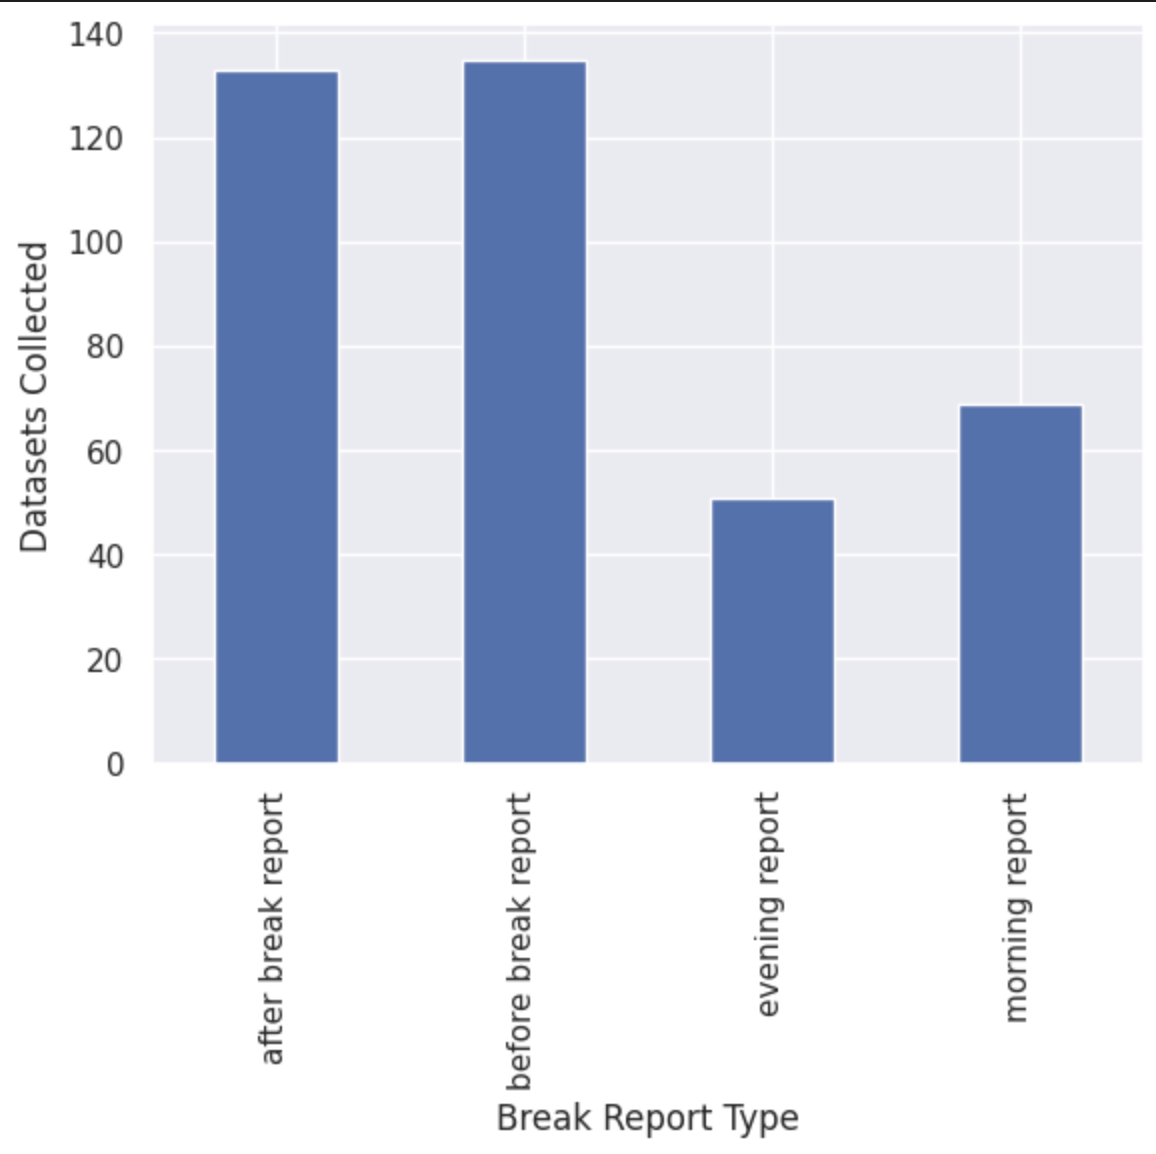
\includegraphics[width=6cm]{hasel_thesis/images/overall_reports.png}
    \caption{Graph of the total reports collected during the intervention}
    \label{fig:overall_reports}
\end{figure}

All participants reported up to 140 breaks during the intervention period.  The after-report number is slightly lower; some participants might forgot to complete the end-break report after their break.  Over 40 evenings and over the 60-morning reports were collected, in which each participant reflected on their current personal resources and used resources.  

The data conducted in the post-questionnaire shows that the participants reflected more on their personal resources, which helped some of them to reflect on their use of resources and how to act on them.  In figure........, it can be shown that the participants did reflect more on their personal resources than before the study.  During the intervention, most of them (11x) reflected multiple times a day, which helped them to reflect on their personal resources and learn what influences them: "These types of questions force me to be mindful about my resources." -[S11,AW]. The reflection and the increase of awareness help some of them (9x) to react if the resources are low or high on how they spend their personal resources: "It works very well since you report it at the moment." - [S01,AW]. More than 50\% agreed on having learned something about their personal resources with the help of the Break schedule.  Specifically, the morning and evening reports were used by many (8x) users for self-reflection purposes: "The reports in the morning and evening were really good for self-reflection on how I felt, which I barely ever do otherwise." -[S06,AW]. 

---------- add the sum of the agreement graph -----------




\textbf{Awareness of Beneficial Breaks.} \label{beneficial_breaks}
When asked about the activities chosen in breaks before the intervention week, the participants try to actively engage in activities which are beneficial for them. However, some participants (4x) do not proactively choose beneficial breaks, as well as others (7x), only sometimes activity engage in beneficial breaks. 
 
----- show graph of if they engage in break activities give you energy etc ---------------------


The before and after break report was perceived positively and useful for reflecting on personal resources by most users as shown in figure ........ The Break Scheduler could help learn about activities which are good as well as activities which do not help by providing the self-report questions before and after the break and showing the experience values of a certain activity on the activity page. As described in the Design of the Break Scheduler, the short self-report before and after each break where split into the three values energy, attention and physical well-being, which was well perceived by some participants: “I very much liked how the personal resources were split up into 3 different dimensions. Usually, I would think of myself in one dimension: "tired" or "energized". During the study, I would map physical aches such as a sore throat, tired eyes, or tension to "body", and mental exhaustion to "attention". The third category, "energy", was the overall feeling at the moment combining the mental and physical aspects.”- [S15, W]. The increase in the awareness of personal resources helped some users to act accordingly: “During the day when I felt tired/exhausted I thought about if it might be more effective to take a break to be more efficient again afterwards.”-[S06, W]. Therefore, it can be shown that the awareness of personal resources had a positive effect on the awareness of the user on beneficial breaks.

It can be conducted that the awareness of the personal resources of the user did increase after the intervention week, which shows the positive effect of the Break Scheduler. The morning and evening report enforces a reflection over the whole day, while the before and after break reports focused on the personal resources which were recharged or used during break activities. From this follows that:

\begin{tcolorbox}[colback=white!5!white,colframe=black!75!black]
  Self-reporting personal resources multiple times a day creates more awareness, helps to be more mindful about how to spend the limited personal resources and helps the user to find beneficial break activities. 
\end{tcolorbox}

\section{Pro-active planning of breaks} \label{planning_breaks}
\begin{comment} 
Pro-active planning of breaks helps to be more mindful of them and helps to give more structure to the day (RQ1, RQ2, RQ3)
\end{comment}

From the pre-questionnaire, it can be concluded that most of the participants (12x) do not plan their breaks in advance and are not taking regular breaks. "I had no break habits before.”-[S10, EM] as one participant stated. All participants do have time periods during which they can plan within day breaks; however, only two participants mentioned in the pre-questionnaire that they plan breaks in advance. These two mentioned they either have fixed team breaks or arrange breaks with others through chat. In figure ----, it can be shown that the number of breaks during the day varies. About half of the participants take two, and one lunch breaks a day. Others (4x) take more breaks than that, but a group of participants take only lunch breaks (3x). Stille, many (9x) are referring to feeling tired and sleepy at the end of the day. This shows that their resources are depleted and need recharging. As discussed in the Background section \ref{background}, one way to do this is by taking regular breaks.

After the intervention period, many participants (9x) took more breaks, and some stated that planning the breaks in advance is one of the key features of the break scheduler as the breaks got more intentional and helps with "remembering that breaks as a concept exist.”-[S11, EM]. One participant mentioned: “So overall, I took more breaks. But I would say that I took longer breaks before as well. And only through this tool, I realized that this was a good thing.”-[S15]. Even though some (5x) mentioned that they took fewer or shorter breaks, the breaks which were taken, were more intentional: “My breaks got more intentional with the Break Scheduler, and I actually took some time to do something beneficial and was then more concentrated again afterwards so I did not have to take a mini-break sooner again.”- [S06, BF], “I undoubtedly took more breaks. But I believe they stayed around the same length. With being more rested, I do believe I have fewer 2 hours scrolling through social media sessions, so shorter.”- [S11,BF] or “I think I took breaks with more awareness: When it said to take a break, I might have talked or walked around or something anyway, but now I actively thought of it as a break.”-[S17,BF]. The scheduling of the breaks into their calendar also helps some participants to be more disciplined with taking breaks: “The Break Scheduler helps me staying disciplined when it comes to taking breaks”- [S04, BF]. Most participants (10x) mentioned that using the Break Scheduler did not impact their work or work environment. One person even mentioned that he gets more things done with the Break Scheduler in the morning: “I got more work done in the morning” –[S04]. Planning breaks ahead helps many (8x) to be more mindful about taking regular breaks. Additionally, some (4x) appreciated the fact that the scheduling of regular breaks helps to structure their day: “It sets my whole working day under a clear structure which sometimes can be hard to follow. Because of the tool, I did more breaks.”-[S13, EM] or “Definitely improved my break habits. And during the two off days, my breaks were quite messed up. And it's even helpful when you can't stick to the schedule perfectly.” – [S15, EM]. The feature of rescheduling breaks also helps to adjust the breaks during the day: “It gives me some structure but doesn't enforce it due to the fact that it's possible to move pauses around.”-[S13, FN]. Nonetheless, planning the exact time and duration of breaks in advance can also lead to inflexibility during the day, as the breaks need to be rescheduled: “I took more breaks, but often had to skip them or move them around” –[S00, EM], “In the afternoon normally I might have taken more breaks but the scheduler told me not to.”-[S17, EM] or “The process itself was not, but sometimes it was a little annoying to change the schedule 3 times a day when you haven't had the chance to take the break when originally planned.”-[S10, FP]. Therefore, the Break Scheduler could be improved by redesigning the rescheduling process. The main factors why participants did not take a break are shown in figure ------. High workload, the timing didn't fit or they didn't see the notification was mentioned most often: "I think it helped me be mindful of taking breaks and highly increase the rate of breaks I took. Nevertheless, I was too often choosing to ignore the break, in favour of a task or project that was approaching a deadline." -[S11]. Even though not all participants could take more breaks due to the mentioned reasons above, it helped them be more aware that they should take more breaks: “It reminded me that I SHOULD take more breaks and take more care of myself.”-[S02]


 ---------- add the figure of reasons why people did not take a break

To sum up, the Break Scheduler helped the participants to plan regular breaks into the work day, which increases the awareness of breaks and forces the user to structure his work day in advance, which helps some of them to have an overall better work structure during the day. The following statement can be concluded:

\begin{tcolorbox}[colback=white!5!white,colframe=black!75!black]
 Proactive planning of breaks helps to be more mindful of them and helps to give more structure to the day.
\end{tcolorbox}
\section{Notification}
\begin{comment} 
Notification helps to raise awareness and remind users to take breaks (RQ1, RQ2, RQ3)

Quantitative:


Qualitative:
- only regular lunch break through most participants (8x) is a lunch break
- Some 
- other than that most take irregular (4x) or only necessary breaks (3x). 
Some do take 

\end{comment}

Some of the participants do not take regular breaks, also since they are not reminded to take any breaks. As stated in the Background section \ref{background}, knowledge workers often forget to take breaks and overwork themselves. This is also the case for some of the participants. As already stated in figure ----------, most participants did not take any regular breaks except the lunch break.

Interestingly, in the post-questionnaire, the notification was mentioned (8x) as the most valuable feature of the Breaks Scheduler for reflecting on break habits. Additionally, many participants (8x) stated that the notification helped them to be reminded about breaks: “Notifications reminded me that I had not taken a break and that maybe I should.”-[S17,AK], “The notifications were really good when working on the computer anyways as I did not have to keep track on time, but actually got a notification.”-[S06,AK] or “The notifications reminded me most that I should take a break (they interrupt my workflow otherwise I wouldn't even think of it)” –[S11,AK]. The reminder notification from the calendar itself was an additional reminder which also helped one participant to push through his tasks in order to complete them before the break: “I liked that breaks were synced with my calendar and oftentimes, the calendar notifications (event coming up in 30 minutes) helped me to push through a task. I would know that I deserved a break according to calendar/bScheduler if I sticked through.”-[S15, FN]. On the other hand, the notification also enforces a specific timing, making it inflexible, which was unfortunate for some (1x) participants. While some prefer to have fewer reminders, others (1x) like to have even more reminders to enforce the action for a break when the work demand is high: “The more notifications I get, the more I can be reminded of taking a consciously taken break. It would have been nice to have more reminders/ notifications on my phone and laptop. One was not enough to get me focused on my break and personal resources.”-[S02]

-----show feature graph-----------


To conclude, the notification of the Break Scheduler helped many participants to remind taking breaks which helped them to be more aware of their break habits. It can be stated:

\begin{tcolorbox}[colback=white!5!white,colframe=black!75!black]
  Notification helps to raise awareness and remind users to take breaks.
\end{tcolorbox}




\section{Improvement personal resources} \label{resources}
\begin{comment} 
Taking more beneficial breaks improves the personal resources levels of the participants (RQ2, RQ3)
\end{comment}

In the pre-questionnaire many participants mentioned they feel often tired or sleepy after a work day, while not most of the breaks are not actively chosen to recharge their personal resources. In figure ----------, most participants stated (9x) they feel often tired or sleepy at the end of the day, whereas only one disagreed with this statement. As also discussed in section \ref{beneficial_breaks}, many participants are not always proactively choosing beneficial breaks. About half of the participants can feel how their personal resources deplete over the course of the day: “Almost without exception they continually decrease until end of workday when i can recover some of them through personal activities. morning activities ameliorate this problem somewhat.-[S00] or “I can feel my personal resources depleting during work sessions by noticing that I am very easily distracted or not able to concentrate on a task.”-[S03] and this can affect their social skills: “I can feel that if I get tired I feel less the need of talking to people. Additionally my skills to verbally express myself decrease.”-[S13]. However, many participants also state that the depletion also depends on the tasks they are working on as well as their motivation: “However, personal resources also depend on the tasks and how motivated I feel to do them.”-[S06]. “Certain activities consume resources, others recharge them. A good day incorporates balancing this shift.”- [S06]. In the pre-questionnaire, many participants already knew some activities which are beneficial for them but need some motivation to do them. More than half (8x) mentioned body movement or (6x) going outside: -	“Sometimes I do sports during my lunch break, but that needs some motivation and mostly some other people that join otherwise I normally don‘t do it.”-[S10] or “Yes, going outside, since you have to get ready.”-[S03]. But also relaxation activities such as (5x) meditation or (2) reading can be beneficial for some of them, but need some initial motivation to do them: “Yes, Meditation often gets lost in the trouble of the day despite it helping me a lot”-[S00] or “Reading/Meditating are also activities that require some initial motivation for me and I don't typically do them all that often.”-[S15]

-------------- for her nach her sleepy tired graph mit 2 linien-------

After the intervention period, when the awareness of beneficial breaks increased, as shown in section \ref{beneficial_breaks}, many participants felt less tired and could see an increase in their energy, attention, and physical and mental well-being. Figure ------ shows that only less then half (5x) agreed, they feel often sleepy and tired, whereas now 6 participants disagree. But not only an overall effect can be stated but also a small effect on the measured key aspects: energy, attention level and physical and mental well-being. Figur --- shows that there is a small increase after the intervention period in all of these areas. ADD MORE TEXT TO STATISTIC WHEN DONE. Ad stated in the section \ref{activities_difference}, there is no one activity most beneficial for all participants, but rather different activities, depending on their preferences. Therefore, the Break Scheduler wants to help the participants to find new beneficial activities. Some participants (3x) got aware that social breaks or breaks where they are going outside are beneficial breaks for them: «Social interactions help me recharge my personal resources, i didn't know that before»-[S04,CK] or «Making the effort and going outside to get some fresh air is worth it. I feel energized after and my attention is much improved.»-[S03, CK] One person learned that breaks with domestic tasks are not considered as a break, as it feels like another work and does not recharge the personal resources: «I do not like to do different work for my breakes like doing domestic tasks or socializing, which all takes energy. I want to do something where no energy from my side is needed, otherwise it doesn't feel like a true break for me, but just different "work".»-[S01, CK]. Not only is it important to know what activities are beneficial but also what activities are not. Most participants (8x) could learn something about activities, which are not beneficial. The most named activity was spending time on their phone (4x): “Beeing on my phone (staring into another screen) during my breaks is definitely not increasing personal resources.”- [S06, DK]. Other unbeneficial activities mentioned are domestic tasks or exercising. 

The Break Scheduler could help the participants to find more beneficial breaks, which helped them to recharge their personal resources and increase their energy, attention, and physical and mental well-being. To sum up, the following sentence can be stated:

\begin{tcolorbox}[colback=white!5!white,colframe=black!75!black]
 Taking more beneficial breaks improves the personal resources levels of the participants.
\end{tcolorbox}


\section{Personal Break Habits}
\begin{comment} 
Self-reporting personal resources multiple times a day creates more awareness, helps to be more mindful about how to spend the limited personal resources and helps the user to find beneficial break activities (RQ1, RQ2, RQ3)
\end{comment}
One key element shown by the collected data is the diversity of preferences of the user. To get a better overview of the personalization of break habits, two subjects will be discussed: timing and duration, as well as activities during the break.


\begin{figure}[htp]
    \centering
    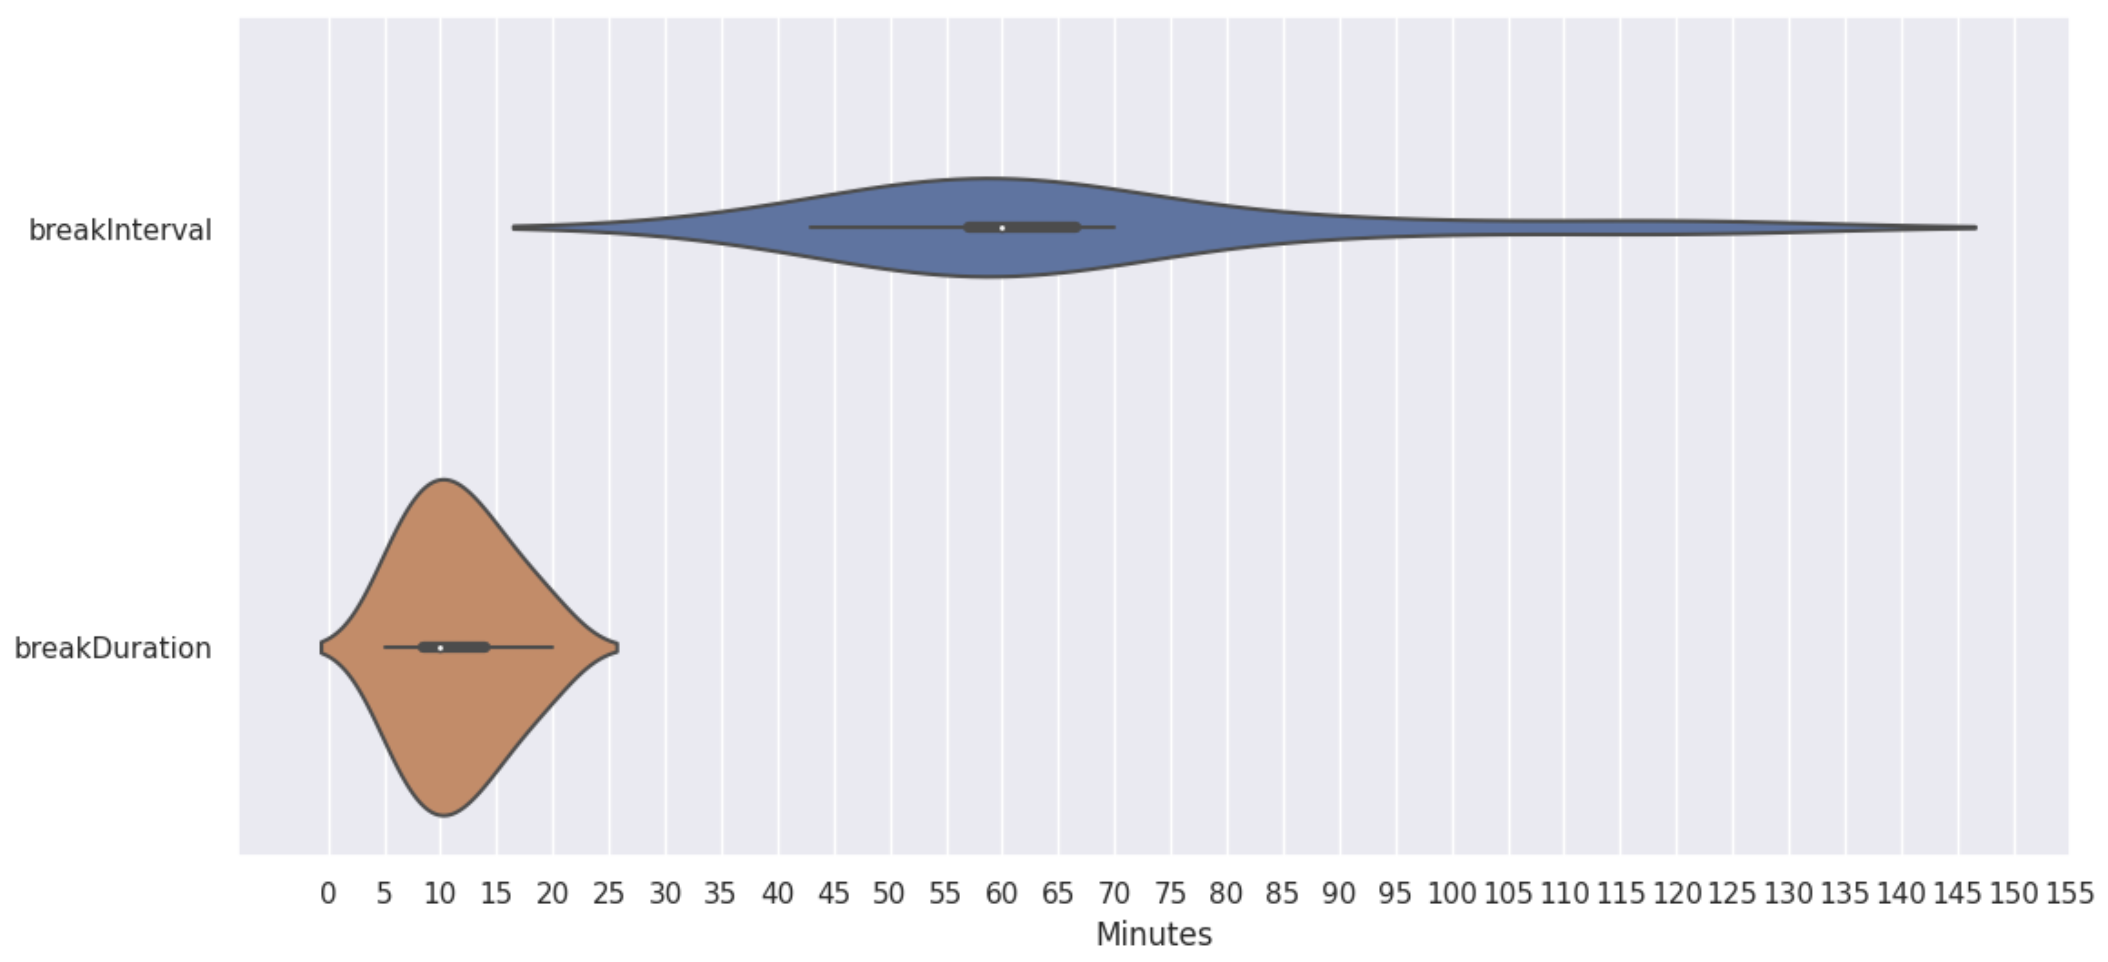
\includegraphics[width=14cm]{hasel_thesis/images/break_Interval_Duration.png}
    \caption{Distribution of the different break intervals and duration according to the database interformation}
    \label{fig:interval_duration}
\end{figure}


\subsection{Timing and Duration}
The collected data can show that the preferences regarding break interval and break duration differ from person to person and depend on different circumstances. Most participants (12x) have high or normal job control, enabling them to plan their tasks and breaks freely. Additionally, most of them (11x) feel supported by their employer to take breaks during working hours, which leads to a solid fundamental to creating regular break habits. For the break interval, some (8x) could state a rough interval, while others (4x) could not state any interval. However, some participants also had an idea but could not state an interval. About half of the participants stated that it strongly depends on the circumstances: "Really depends on a lot of factors. Like how motivated I am, how well rested I am, how close the deadline is, the weather,...”-[S06] or -	“I don‘t have a special focus time I would say. I think it depends more on the task. I have to get into a task and when I am really working on something, I often want to finish this task if possible.”-[S10]. Similar behaviour was reported for the duration. Some (8x) of the participants could state a rough duration number which can differ between 10-15 (2x), 15-30 (2x) and 45-60 (1x) (for a lunch break). One participant stated: “I guess a ten-minute break is enough. For sure the duration depends on my mood and the tasks I have to do.”-[S13] while another mentioned: “The longer the better. Maybe 30 minutes as a minimum.”-[S15] Around 5 people could not state any fixed break duration and stated that it depends on the situation or other aspects, as if they take a break alone or with others. “If I am by myself breaks are usually shorter as I get bored after a while. But in a social setting, the length depends a lot on the situation.”-[S06, AV]. This can also be stated by the fact that most (10x) participants agreed that the break duration is dependent on certain circumstances, whereas a minority (3x) didn't think so. -Most of the mentioned factors are Time of the day (2x), mood(2x), tasks (2x), and interruption for example open office space, but also the menstrual cycle or the food and beverage intake. “It depends on the task I am working on, some tasks require more concentration or attention.”-[S03]. “Ideal would be until the task is done, then a break and afterwards continue with the next task, so yes it does depend.”-[S06]. An important factor which was mentioned (3x) is motivation. If the motivation is high, the break interval is mostly longer: “Motivation oft plays a major part. High motivation can significantly extend attention while the lack thereof can inversely necessitate longer breaks.”-[S07]. Some participants could also already feel the need for higher breaks after an extended focus period: it depends on “.. how burnt out I am from working on high focus for longer periods of time (that's when I'm usually in need of holidays)”-[S02].

---------------- add agreement graph --------


After the intervention period, most participants (9x and 2-unanswered) could learn something from the Break Scheduler regarding their break habits. Some (2x) could find out that they need to take more breaks, and others (3x) could figure out they need to take more different breaks. 7 out of 13 could learn something about their break duration, while 8 of 13 could learn something about their preferred interval. Figure \ref{fig:interval_duration} shows the collection of the selected break interval and duration of the participant to schedule their breaks during the intervention period. It appears that the distribution of the break interval is large among the participants (between 147min and 17min). This can also be strengthened by the post-questionnaire data. About half of the participants (6x) could state a specific break interval which does not deplete their resources too much and enables them to work focused. Some mentioned their preferred interval is 50min (2x), other 60min(2x) or 90min(2x). The average of the selected break interval is 60min. Four participants mentioned that they do not have one preferred interval, as it depends on certain circumstances as the tasks they are doing: “I feel like this is quite situational for me, mostly depending on the task. A task I really like doing and am totally focussed on, I can do for longer. When doing a task  I like less, my time of attention is less, and it might make sense to take breaks more frequently.”-[S06] or the daytime (2x): “Mornings longer, i.e. 1.5-2h, in the afternoon more around 50min”-[S00]. One effect of the break interval is the ability to resume work after a break. Some participants (2x) explicitly mentioned, they like to have longer intervals, as they have problems resuming work after a break: "I don't like taking lots of breaks, because when I am in working mode, taking a break takes me completely out of it and it is hard to get into this mode again after the break."-[S01]. On the other hand, for some people, it helps to regain attention for tasks: “Yes, a duration of 50 minutes has worked well for me. It is useful to take breaks even if I am still on a task, to regain attention.”- [S03]. Differences also appear in the duration. From figure \ref{fig:interval_duration}, it can be concluded that break duration does not as much diverge as the interval. The selected break duration stays between .... and 25min. The average of the selected break duration is 10min. When asked about break duration, most participants, except one, could find a preferred break duration. However, this duration does differ. About half of the users (6x) like to take longer breaks (15min or longer), while only two people like rather short breaks (less than 15min): “15 min generally shows the best results. Less time can result in not sticking to the schedule.”-[S07], “I definitely think breaks can be too long and can also kick you out of focus. Therefore, in my case, I think the chosen break interval of 20min was very good.”-[S10] or “Generally, I learned that breaks are more useful when they are longer (at least, on days when the overall energy level is already quite low from the start).”-[S15]. A bigger group of participants (5x) mentioned they liked to mix their break duration during the day: “I like shorter breaks of 5 for activities like coffee break, socializing, surfing on the internet,... because if longer, I feel like I am "too far away" from work after the break and it is more difficult to start again. For breaks like going outside and taking a walk, longer breaks are better for me as I am able to completely get my brain off of work and return with a "fresh" brain.”-[S06] and others stated that it strongly depends on the activity during the break: “Again, I found that the break duration needed varied. Of course, it also varies with the break activity!”-[S17] or break categories: “I like long social breaks and short active breaks.”-[S09].

The personalisation of the timing and duration in the Break Scheduler is, therefore, a key factor and needs to have features supporting the participants in doing this. One feature is ht adaptation of the interval and duration, which helps the user to optimize his break habits and will be evaluated each evening. 10 out of 11 stated that these features helped them to adjust to their needs. The integration of the schedule into the calendar was also mentioned (4x) as helpful in adjusting the timing or duration: “The app gave me good ideas, a suggestion on what breaks to take at a certain time. It could not help me with my irregular work schedule.”-[S02 ]. However, following the suggested timing and duration is difficult if you have an irregular work schedule and low job control: " As explained above. The app gave me good ideas and suggestions on what breaks to take at a certain time. It could not help me with my irregular work schedule."- [S02] 

Add some more info to what they have learned about their break habits. Add also -	“I would need a system that doesn't enforce taking breaks as strictly in terms of the timing.”-[S15,AK]
“I tried for the first time doing shorter but more breaks with the break scheduler, but this doesn't work for me at all. With the break scheduler I could confirm that few, long breaks are the best option for me.”- [S01, BF]
 

\subsection{Break Activities} \label{activities_difference}
The types of activities people prefer during their breaks can vary greatly, not just in terms of when and how long they take breaks. The pre-Questionnaire data shows that preferences diverge when looking at the break activities. Many (7x) mentioned that body movement helps them to recharge their personal resources, while others (4x) prefer nutritional intake. All categories used by the Break Scheduler were stated as most beneficial for recharging the personal resources by at least one participant. Interestingly, in the pre-questionnaire, most mentioned break activities were activities done before the start of the day, during the lunch break or after the work day, but barely within-day break activities: “Body movement followed by meditation in the morning allows me to stay concentrated and alert most of the morning, which makes them my most productive times.” –[S00],  “I take the longer path in the morning to get from public transport to the building, which kind of wakes me up.”-[S06] or -	“I usually do some type of sport once a day for about an hour. Either outside or inside. Mostly early in the evening after returning from the office. During home-office, I may take the break earlier." - [S15]. 

ADD MORE TEXT TO ACTIVITIES FROM QUESTION: Are there breaks that are successful at recharging your personal resources, but take some motivation to pursue? If so, which ones?

After the intervention, participants learned something about their preference for break activities or categories. This could be concluded by the post-questionnaire data, which is shown in figure .......... More than half of the participants (12x) agreed that the suggested activities by the Break Scheduler are beneficial to restore their personal resources and activities they like. It also helps the participants (12x) to choose beneficial activities proactively: “Through the app, I was motivated to do more of the good breaks.”-[S09,T] or “I like that I did not have to choose the activity... It made a good decision for me :)”- [S09,AK]. The Break Scheduler could also help participants to find new break activities: “It also gave me new inspiration for activities during breaks and showed me that not every activity is equally recharging my resources.”-[S06,T] or “I (actually) already knew which breaks are good for me (I was still doing them), but I learned about some more good ones like stretching.”- [S09, T]. When looking at experience values of the activities of each user, figure ........ shows that there exists no "perfect break activity" fitting for all users. ADD SOME TEXT TO STATISTICS OF ACTIVITIES



\begin{tcolorbox}[colback=white!5!white,colframe=black!75!black]
 Break habits are very personal and differ from person to person. A tool supporting the user to create a beneficial break habit should enable personalization.
\end{tcolorbox}


\chapter{Discussion}

\subsection{Threats to validity}

\subsection{Futur work}

\chapter{Conclusion}
\textcolor{red}{not yet finished}
%
- short summary
- conclusion
    - show limitations



Another factor influencing the break interval is the user's sleep schedule. As shown in several studies \cite{Rosekind.2010} \cite{Gingerich.2017} \cite{Choi.2018}, a good night's sleep  can help to stay focused longer, which means taking fewer breaks. 
It is also important to ensure that the system does not suggest breaks to the user during periods of high concentration and focus when suggesting a break, to avoid interruptions and dissatisfaction with the system. Thus, various computer interaction trackers will be used to detect the state of the user and the personal calendar will be considered, to avoid scheduling breaks during meetings. 
To account for breaks that are less predictable, such as when a user is very stressed, the approach shall consider suggesting “emergency breaks” when sensing a higher stress state from an increased heart rate \cite{Hjortskov.2004}. 
Finally, spontaneous breaks that were not suggested by the system must also be detected to help adjust and personalize the timing of future breaks. Detecting such breaks could be accomplished through pedometer data, computer interaction trackers or self-reports. 




% 
% \subsubsection{Subsubsection}
% \fig[.5\textwidth]{logos/logo_hasel}{Our logo}{logo}

% \subsection{Subsection}
% %
% \paragraph{Paragraph.} Always with a point.

% \begin{lstlisting}[caption=An example code snippet]
% /**
%  * Javadoc comment
%  */
% public class Foo {
% 	// line comment
% 	public void bar(int number) {
% 		if (number < 0) {
% 			return; /* block comment */
% 		}
% 	}
% }
% \end{lstlisting}

\appendix
\chapter{First Appendix}
\chapter{Second Appendix}

\backmatter
\bibliographystyle{alpha}
\bibliography{hasel_thesis/references}



\end{document}
